\documentclass[11pt]{article}
\usepackage[margin=1.1in]{geometry}
\usepackage[T1]{fontenc}
\usepackage{amsmath, amssymb, amsthm}
\usepackage{booktabs}
\usepackage{array}
\usepackage{xcolor}
\definecolor{linknavy}{RGB}{25, 55, 125}
\usepackage[colorlinks=true, linkcolor=linknavy, citecolor=linknavy, urlcolor=linknavy]{hyperref}
\usepackage{orcidlink}
\usepackage{fancyhdr}
\usepackage[justification=raggedright,singlelinecheck=false]{caption}
\usepackage{algorithm}
\usepackage{algpseudocode}
\usepackage{tikz}
\usetikzlibrary{arrows.meta, positioning}
\usepackage{pgfplots}
\pgfplotsset{compat=1.16}
\usepackage{placeins}

\newcommand{\numDetF}{-2}
\newcommand{\numBranches}{382}
\newcommand{\numEnumInst}{216}
\newcommand{\numBadResidual}{930}
\newcommand{\numEnumFibers}{648}
\newcommand{\numShapes}{6}
\newcommand{\numRigCases}{648}
\newcommand{\numWeightPairs}{8}
\newcommand{\weightPairs}{(1,0),\ (1,1),\ (2,1),\ (3,1),\ (3,2),\ (4,3),\ (5,2),\ (5,3)}
\newcommand{\numSweepDeg}{5}
\newcommand{\numKillDeg}{19}
\newcommand{\numGrid}{36}
\newcommand{\numGridNoPlane}{27}
\newcommand{\numGridPlane}{9}
\newcommand{\numCensusOne}{5}
\newcommand{\numCensusThree}{1}
\newcommand{\numDcollision}{36864}
\newcommand{\numDetModThirteen}{10}
\newcommand{\numDetModHundred}{98}
\newcommand{\ptModThirteenA}{(6, 5, 8)}
\newcommand{\ptModThirteenB}{(6, 8, 6)}
\newcommand{\ptModThirteenT}{(11, 11, 1)}
\newcommand{\ptModHundredA}{(74, 18, 80)}
\newcommand{\ptModHundredB}{(80, 83, 35)}
\newcommand{\ptModHundredT}{(47, 47, 1)}
\newcommand{\numLemmaCases}{20}
\newcommand{\numBridgeInst}{93}
\newcommand{\numRigidInst}{60}
\newcommand{\numAdmissCond}{5}
\newcommand{\numPatterns}{24}
\newcommand{\numSeedDegMax}{5}
\newcommand{\numDegreeMax}{5}
\newcommand{\numPfiveDet}{-20}
\newcommand{\numWallCuspA}{0.1481}
\newcommand{\numWallCuspB}{1.3333}


\newtheorem{theorem}{Theorem}[section]
\newtheorem{proposition}[theorem]{Proposition}
\newtheorem{lemma}[theorem]{Lemma}
\newtheorem{conjecture}[theorem]{Conjecture}
\theoremstyle{definition}
\newtheorem{definition}[theorem]{Definition}
\theoremstyle{remark}
\newtheorem{remark}[theorem]{Remark}

\newcommand{\C}{\mathbb{C}}
\newcommand{\Q}{\mathbb{Q}}
\newcommand{\R}{\mathbb{R}}
\newcommand{\Gm}{\mathbb{G}_m}
\newcommand{\detJ}{\det JF}
\newcommand{\MV}{\textbf{[MV]}}
\newcommand{\DD}{\textbf{[D]}}
\newcommand{\CC}{\textbf{[C]}}
\newcommand{\VV}{\textbf{[V]}}
\newcommand{\UU}{\textbf{[U]}}

% Page-1 header block (conventions/manuscript-header-standard.md). The four document
% macros are set by the publishing tool when the version DOI is reserved. At this text
% width the two DOIs do not fit on one line of the box, so each has its own line.
\newcommand{\doctype}{Preprint}
\newcommand{\docversion}{v0.15}
\newcommand{\docdate}{14 November 2026}
\newcommand{\versiondoi}{10.5281/zenodo.24226224}
\newcommand{\conceptdoi}{10.5281/zenodo.21503365}
\newcommand{\docrepo}{github.com/fsantibanezleal/CAOS\_RESEARCH}

\newcommand{\headerblock}{%
\begin{center}
\fbox{\parbox{0.94\textwidth}{\small\raggedright
\textbf{\doctype} \quad$\cdot$\quad \docversion, \docdate \quad$\cdot$\quad Licence CC BY 4.0\\[2pt]
CAOS Research open-problems programme \quad$\cdot$\quad problem \texttt{jacobian-conjecture}\\[2pt]
Version DOI \href{https://doi.org/\versiondoi}{\texttt{\versiondoi}}\\[2pt]
Concept DOI (always latest) \href{https://doi.org/\conceptdoi}{\texttt{\conceptdoi}}\\[2pt]
Not peer reviewed. Source code, data and computational records: \href{https://\docrepo}{\texttt{\docrepo}}
}}
\end{center}
\vspace{4pt}}

\title{The Three-Dimensional Counterexample to the Jacobian Conjecture:\\
Exact Validation, a Proved Seed-Family Constructor,\\
the Discriminant Wall of Non-Properness,\\ and Planar Equivariant Rigidity}
\author{Felipe Santib\'a\~nez-Leal\,\orcidlink{0000-0002-0150-3246}\\
\small CAOS Research program, \texttt{github.com/fsantibanezleal/CAOS\_RESEARCH}}
\date{\docdate}

\pagestyle{fancy}
\fancyhf{}
\fancyhead[L]{\small CAOS Research \doctype}
\fancyhead[R]{\small Jacobian Counterexample: Foundations \textperiodcentered\ \docversion}
\fancyfoot[C]{\small \thepage}
\renewcommand{\headrulewidth}{0.4pt}
\fancypagestyle{plain}{\fancyhf{}\fancyfoot[C]{\small \thepage}\renewcommand{\headrulewidth}{0pt}}

\begin{document}
\maketitle
\headerblock

\begin{abstract}
On 2026-07-20, Levent Alp\"oge announced (crediting the language model Claude Fable 5) % voice-ok: external attribution, as the announcement states it
a polynomial map $F : \C^3 \to \C^3$ with constant Jacobian determinant $-2$
and a repeated value, refuting the Jacobian conjecture for every $N \ge 3$. The
fiber over the announced target consists of exactly the three announced points.
The map is a weighted skew product over the invariants $v = xy$, $t = x^2 z$; its Keller property is a
two-variable identity. We prove a
constructor: every admissible seed polynomial $p$, scale $k$ and section $q$ gives a Keller map of
determinant $-k\,p(1)^2$ and generic fiber degree $\deg p + 1$. The degree law $(5d-3, 5d-4, 4)$ is machine-verified on four seeds; its extension
to every seed and the minimality of the announced map within the family are conjectural.
The asymptotic variety of $F$ is the discriminant surface $27A^2C^2 - 18ABC + 16A + B^3C - B^2 = 0$
alone. $F$ is not surjective, over $\C$ or $\R$: its image omits an explicit curve, and the fibers over $C = 0$ have three points
off $B^2 = 16A$ (computation EXP-145). Version 0.14 stated a surjective real restriction and an asymptotic plane $C = 0$, both false, and the minimality of the announced map as proved, which is conjectural. % voice-ok: correction notice required for a published statement
In dimension two, equivariant
Keller maps are linear for opposite-sign weights and affine, $(f_0 x,\, g_0 y + c)$ or its swap, for one
zero weight, so a planar counterexample must be non-equivariant.
\end{abstract}

\section{Introduction}

Let $k$ be a field of characteristic $0$. A polynomial map $F = (F_1, \dots, F_N) : k^N \to k^N$
is a \emph{Keller map} if $\detJ$ is a nonzero constant. The Jacobian conjecture $JC(N)$,
stated in two variables by Kraus in 1884 (with a flawed proof whose gap, control of ramification
at infinity, remained the subject's central obstacle \cite{Rodriguez2026}) and popularized by
Keller in 1939 \cite{Keller1939}, asserted that every Keller map has a polynomial inverse. Over
$\C$, invertibility is equivalent to injectivity, so a refutation requires exactly one repeated
value. The conjecture is Problem 16 of Smale's list \cite{Smale1998}. The positive results and
reductions that surrounded it (Section~\ref{sec:related}) never bounded the search in dimension
three, which is where the refutation was found.

On 2026-07-20, Alp\"oge announced the map, with $u = 1 + xy$,
\begin{equation}\label{eq:F}
F = \bigl(\,u^3 z + y^2 u (4 + 3xy),\;\; y + 3x u^2 z + 3x y^2 (4 + 3xy),\;\; 2x - 3x^2 y - x^3 z\,\bigr),
\end{equation}
with $\detJ \equiv -2$ and
$F(0, 0, -\tfrac14) = F(1, -\tfrac32, \tfrac{13}{2}) = F(-1, \tfrac32, \tfrac{13}{2}) =
(-\tfrac14, 0, 0)$ \cite{Alpoge2026}. Appending identity coordinates refutes $JC(N)$ for all
$N \ge 3$; the case $N = 2$ remains open. The announcement consists of the map and its
collision, both machine-checkable. This paper studies the map itself: its validation, its
structure, the family of Keller maps that the same mechanism generates, the geometry of its
non-properness, its real image and fibers, its reduction modulo primes, the weight systems on which
the mechanism can and cannot be repeated, and two-dimensional equivariant rigidity as the bridge to
the planar case. Two companion papers continue the programme: the planar paper \cite{SLplanar}
develops the machinery for $JC(2)$ and the cascade paper \cite{SLcascade} derives the consequences
of the counterexample for related conjectures.

The contributions are the following.
\begin{itemize}
\item An exact validation of the map and its full fiber, with a hand-checkable substitution (Section~\ref{sec:valid}).
\item A proof of the Keller property, of the reconstruction of preimages and of the generic fiber degree for a
family of maps indexed by a seed polynomial, a scale and a section, with rational collisions in fiber degrees $3$ to $6$ and an
explicit statement of what the machine verification of the degree law covers (Section~\ref{sec:family}).
\item The exact asymptotic variety of $F$, the structure of its fibers over the plane $C = 0$, the complement of its image and its
real census (Sections~\ref{sec:asymptotic} and~\ref{sec:real}).
\item A proof that $\Gm$-equivariant planar Keller maps are linear for opposite-sign weights and affine for one zero weight
(Section~\ref{sec:rigidity}).
\item An ablation of the mechanism on other weight systems (Section~\ref{sec:ablation}).
\end{itemize}

Each computer-assisted result cites the archived computation that establishes it as EXP-$nnn$ (see
Section~\ref{sec:repro}). Each result is labeled \MV{} (machine-verified exact identity or exact
computation), \DD{} (derived analytically; certified on instances where stated) or \CC{} (conjecture).
Statements about the literature carry \VV{} (read in the primary text) or \UU{} (not confirmed in a
primary source). The paper is organized as follows: related work (Section~\ref{sec:related}), the problem
and notation (Section~\ref{sec:problem}), the computational methods (Section~\ref{sec:methods}), the
experimental design (Section~\ref{sec:design}), the results on the map and its family
(Sections~\ref{sec:valid} to~\ref{sec:asymptotic}), the two-dimensional results (Section~\ref{sec:planar}), the ablation, the validation, the
discussion and the limitations.

\paragraph{Correction of version 0.14.}% voice-ok: correction notice required for a published statement
Version 0.14 stated three results that are corrected here. (i) It stated that the announced map restricts to a surjective real Keller map; this is false, because the fiber over every point of the curve $\Gamma$ of \eqref{eq:gamma} is empty, over $\C$ and over $\R$, and the image is $\C^3 \setminus \Gamma$ (Theorem~\ref{thm:realcensus}). (ii) It stated that the plane $C = 0$ is part of the asymptotic variety and that a generic fiber over it is a single point; this is false, because the fiber over $(A,B,0)$ has three points when $B^2 \neq 16A$ and the asymptotic variety is the surface $\{\Sigma = 0\}$ alone (Theorems~\ref{thm:cplane} and~\ref{thm:asymptotic}). (iii) It stated that the announced map is the smallest member of its family; this is now Conjecture~\ref{conj:degrees}, since the degree law is machine-verified on four seeds only. Computation EXP-145 certifies (i) and (ii). % voice-ok: correction notice required for a published statement

\section{Related work}\label{sec:related}

\subsection{Reductions and positive results}

Wang proved the conjecture for maps of degree two in every dimension \cite{Wang1980}~\UU{} (the
theorem's text was not read in the primary source; the bibliographic entry is complete). The announced map has degree
$7$, and the instances of Section~\ref{sec:family} have degree vectors that all dominate $(7,6,4)$, so Wang's theorem is the only
general degree floor for $N = 3$ used in this paper. Bass, Connell and Wright reduce the conjecture in all dimensions to maps
$x + H$ with $H$ cubic homogeneous \cite{BCW1982}~\VV{}; the reduction adds variables, so it neither bounds the search in
dimension three nor carries $F$ to a fixed small dimension. Dru\.zkowski reduces further to the cubic-linear form, in which each
$H_i$ is the cube of a linear form \cite{Druzkowski1983}. De Bondt and van den Essen show that it suffices to treat cubic
homogeneous maps with symmetric Jacobian \cite{dBvdE2005}~\VV{}, and Zhao shows that the conjecture is equivalent to a vanishing
conjecture for Hessian nilpotent polynomials \cite{Zhao2004, Zhao2007}. Keller proved the birational case
\cite{Keller1939}. Van den Essen's monograph \cite{vdEssen2000} collects these results together with the structure theory of
polynomial automorphisms used below.

\subsection{The planar case}

For $N = 2$ the evidence is arithmetic and geometric. Magnus proved that a Keller map whose component degrees have greatest common
divisor $1$ is an automorphism \cite{Magnus1955}; Appelgate and Onishi and Nagata extended this to a greatest common divisor at most
$8$ or prime \cite{AppelgateOnishi1985, Nagata1989}, as relayed in the surveys read for this work. Heitmann showed that a counterexample has
$\gcd(\deg P, \deg Q) \ge 16$ \cite{Heitmann1990}, and Abhyankar proved further restrictions on the greatest common divisor in a long
analysis of Newton polygons \cite{Abhyankar2008}. Guccione, Guccione and Valqui give an elementary proof of the bound $16$, exclude
$2p$ for a prime $p$ and analyse the case $16$ in detail \cite{GGV2017}~\VV{}. Moh excluded counterexamples of degree up to $100$ by
approximate roots, with a complete published proof only for the smallest of his four exceptional degree cases \cite{Moh1983}~\VV{}; the
same group raised the floor to $108$, leaving the single degree pair $(72,108)$ undecided \cite{GGHV2017, GGHV2022}~\VV{}, and an exact
computer-assisted exclusion of that pair, conditional on their reduction, is claimed in \cite{Helali2026}. Makar-Limanov constrains the
Newton polytope of a minimal counterexample \cite{MakarLimanov2021}~\VV{}. Kanel-Belov and Fedorov show that $JC(2)$ implies a generalized
Dixmier statement for the first Weyl algebra, without announcing a counterexample \cite{KanelBelovFedorov2026}~\VV{}. None of these
results touches the symmetry class studied here; Section~\ref{sec:planar} shows that class is closed in dimension two.

\subsection{Real, positive-characteristic and equivariant results}

Pinchuk refuted the strong real conjecture by a locally invertible planar map with non-constant Jacobian \cite{Pinchuk1994}; the
constant-Jacobian real statement in dimension three falls with the same example as the complex one (Section~\ref{sec:real}). In positive
characteristic the conjecture is classically false through maps such as $x - x^p$, whose degree equals the characteristic; Section~\ref{sec:family}
gives explicit non-injective Keller maps whose degree lies below the characteristic. For equivariant maps in dimension two,
Miyanishi proves that an equivariant \'etale endomorphism of $\mathbb{A}^2$ for a small finite subgroup of $GL_2$ of even order is an
automorphism \cite{Miyanishi2023}~\VV{}. Dubouloz and Palka show that equivariance under $\C^*$ does not rigidify \'etale
endomorphisms on every surface: counterexamples to the equivariant generalized conjecture exist on pseudo-planes exactly for the group $\C^*$
\cite{DuboulozPalka2018}~\VV{}. Shaska classifies all Keller maps of $\C^2$ that are equivariant for a nontrivial $\Gm$-action, in every
signature of the weights \cite{Shaska2026}~\VV{}. The classification of Section~\ref{sec:rigidity} for opposite-sign and one-zero weights
agrees with it and was derived independently; no priority is claimed.

\subsection{The counterexample and its derivations}

The primary artifact is the posted map with its collision \cite{Alpoge2026}. Van den Essen found it again by an elementary search for a
three-variable Keller map $(a + bz,\, c + dz,\, x + x^2y + x^3z)$ with $a,b,c,d \in \C[x,y]$, guided by the reducibility of the third
component, and recalls Magnus' criterion for the planar case \cite{vdEssen2026}~\VV{}. De Bondt homogenizes the map to a map $x + H$ on
$\C^{15}$ with every $H_i$ homogeneous of degree $7$ and reports counterexamples to related conjectures in further dimensions
\cite{deBondt2026}~\VV{}; Thompson gives an explicit cubic-homogeneous form in dimension $24$ \cite{Thompson2026}. None of these derivations proves the Keller property for a family of maps, reconstructs the preimages, or describes where the sheets of the fiber escape; they each start from the announced map and
transform it, and none of them gives a degree law or a rational collision outside the announced map. The consequences for the Mathieu, Dixmier, Poisson and Gaussian moments conjectures are collected in Section~\ref{sec:discussion} and developed in \cite{SLcascade}; the explicit witnesses in other dimensions that
they use are those of \cite{deBondt2026} and of two further works by Long \cite{LongSU2, LongGMC}.

\subsection{Position of this paper}

The constructor of Section~\ref{sec:family} is proved here, together with the reconstruction of preimages that exposes the geometry of
non-properness; a family with the same three conditions on the seed circulates informally, without proof, in a secondary source not cited here~\UU{}, and the scale, the section tail and the
proof are the additions made here. The exact asymptotic variety, the complement of the image and the structure of the fiber over $C = 0$ in Section~\ref{sec:asymptotic}
have no counterpart in the works above. The two-dimensional classification is contemporaneous with \cite{Shaska2026}, which contains it. Against the planar works of Section~\ref{sec:related}, whose methods are arithmetic and Newton-polygon arguments for $N = 2$, the results here
act on a different axis: they show which symmetry class of maps can and cannot produce a refutation, and they supply the exact objects (fibers, discriminant, image) that a proof of $JC(2)$ through properness would have to control. The claims of this paper
are limited to the maps studied; the degree floor for $N = 3$, the planar degree frontier and the status of related conjectures are cited, not extended.

\section{Problem formulation and notation}\label{sec:problem}

We work over $\Q$ unless stated, and over $\C$ or $\R$ for geometric statements. A \emph{Keller map} is a polynomial
map $F : k^N \to k^N$ with $\det JF \in k^\times$. The map $F$ of \eqref{eq:F} is written $F = (P, Q, R)$. A \emph{$\Gm$-action} on $k^N$ with
integer weights $(a_1, \dots, a_N)$ is $t \cdot (x_1, \dots, x_N) = (t^{a_1} x_1, \dots, t^{a_N} x_N)$, and a polynomial map is
\emph{equivariant} if each component is a weight vector: $F_i(t \cdot p) = t^{b_i} F_i(p)$ for integers $b_i$ (the weights of the target
action). The three questions studied are the following.

\begin{enumerate}
\item \emph{Validation.} Is $F$ a Keller map, and what is the exact fiber over the announced target?
\item \emph{Generalization and geometry.} Which maps of the same structure are Keller maps, how do their fibers behave, where do preimages escape to infinity, and what
are the image and the real fibers of $F$?
\item \emph{Obstruction in dimension two.} For which $\Gm$-actions on $\C^2$ does an equivariant Keller map exist that is not an affine automorphism?
\end{enumerate}

Three conventions fix the meaning of the statements. A \emph{fiber} $F^{-1}(a)$ is the set of points of the stated space (over $\C$ unless $\R$ is named) that map to $a$, counted without multiplicity; since $\detJ \neq 0$ every point of a fiber is a regular point. The \emph{generic fiber degree} is the number of points of the fiber over a target outside a proper closed subset of the target space. The \emph{asymptotic variety} $A(F)$ is the set of limits $\lim F(p_n)$ along sequences $p_n \to \infty$ whose images converge; a Keller map is proper over a neighborhood of a target that is not in $A(F)$, and a point of $A(F)$ is a target at which sheets of preimages escape. Exact arithmetic means that every coefficient is a rational number (or a residue modulo a prime) and that equality is tested symbolically.

For the first two questions the data are the polynomials of Table~\ref{tab:notation}. The weights of $F$ are
$(1,-1,-2)$ on the source and $(-2,-1,1)$ on the target, so $v = xy$ and $t = x^2 z$ are the weight-zero invariants
and every component of $F$ is $x^{b}$ times a polynomial in $(v, t)$. For the third question a nontrivial action on $\C^2$ has only one
independent weight-zero invariant. The target of the constructor is the set of
quadruples $(p, k, q)$ for which the lifted map is a polynomial Keller map; the target of the geometric questions is the discriminant surface
and the complement of the image.

\begin{table}[t]\centering\small
\begin{tabular}{p{0.16\textwidth}p{0.78\textwidth}}
\toprule
Symbol & Meaning \\
\midrule
$F = (P,Q,R)$ & the announced map \eqref{eq:F}; $F_{p,k,q}$ is the map of the constructor \\
$u,\ v,\ t$ & $u = 1 + v$; the weight-zero invariants $v = xy$, $t = x^2 z$ \\
$a_1,\ b_1,\ c_1$ & reduced components $x^2 P$, $xQ$, $R/x$; polynomials in $(v,t)$ \\
$V',\ T'$ & output invariants $V' = b_1 c_1 = QR$, $T' = a_1 c_1^2 = PR^2$ \\
$p,\ \Phi,\ d$ & seed polynomial $p$ of degree $d$ with $p(0)=0$, and $\Phi(w) = \int_0^w p$ \\
$k,\ m,\ q$ & scale $k \neq 0$, $m = -k\,p(1)$, and the section $q(v)$ with $q(0) = k$ \\
$s,\ w$ & $s = c_1 = q(v) - t$ and $w = u s / k$ \\
$(A,B,C)$ & coordinates of the target; $V' = BC$ and $T' = AC^2$ over a target \\
$W,\ D,\ \Sigma$ & fiber polynomial $W(w) = k^2\Phi(w) - wBC + AC^2$; its discriminant $D$; the surface polynomial $\Sigma$ with $D = -16 C^2 \Sigma$ \\
$(w_1, -w_2)$ & weights of a $\Gm$-action on $\C^2$; $v = x^{w_2}y^{w_1}$ is the invariant \\
\bottomrule
\end{tabular}
\caption{Notation used for the three-dimensional map and its family. Each symbol is defined at its first use in the text; the table collects them with the polynomial or constant they denote.}
\label{tab:notation}
\end{table}

\section{Computational methods}\label{sec:methods}

\subsection{Software and arithmetic}

Every computation is exact. Coefficients lie in $\Q$ (rational numbers with arbitrary-precision numerators and denominators) or, for the
reductions of Section~\ref{sec:family}, in $\mathbb{F}_\ell$; no floating-point arithmetic enters any result. The software is the computer algebra system sympy,
whose version $1.14$ is named in the archived description of computation EXP-001; the other archived descriptions name sympy without a version. Gr\"obner
bases are computed for the lexicographic order. Univariate real roots are isolated by Sturm sequences, so a root count is a certified integer and not a floating-point estimate. Polynomiality of a rational function is decided by exact cancellation of its numerator and denominator, and identities with symbolic coefficients are decided by expansion to a canonical form and a test for the zero polynomial. The figures of this paper are drawn
from the exact polynomials by the script \texttt{gen\_tables.py}, which also writes every table and every number quoted from an archived output.
The archived outputs record no wall times except that of EXP-145 (sympy $1.14.0$, \numExpSeconds{} seconds); the costs stated below are operation counts.

\subsection{Algorithm A1: exact validation and the full fiber}

Algorithm~\ref{alg:valid} is the validation of Section~\ref{sec:valid}. It separates the pointwise substitution, which is checkable by hand, from the
Gr\"obner computation, which shows that no further point exists in the fiber.

\begin{algorithm}[t]
\caption{Exact validation of a candidate Keller map and the full fiber over a rational target.}\label{alg:valid}
\begin{algorithmic}[1]
\Require $F = (F_1,F_2,F_3) \in \Q[x,y,z]^3$; a rational target $a \in \Q^3$; candidate points $p_1,\dots,p_r \in \Q^3$
\State $J \gets$ the $3\times 3$ matrix of partial derivatives; $\Delta \gets \det J$, fully expanded
\State \textbf{check} $\Delta \in \Q^\times$
\For{$i = 1,\dots,r$} \textbf{check} $F(p_i) = a$ in exact rationals \EndFor
\State \textbf{check} the $p_i$ are pairwise distinct
\State $G \gets$ lex Gr\"obner basis of the ideal $(F_1 - a_1,\, F_2 - a_2,\, F_3 - a_3)$ with $x > y > z$
\State read the univariate eliminant in $z$ and its roots with multiplicity; read the relations of the other basis elements
\Ensure $\Delta$; the conclusion ``$F$ is a non-injective Keller map''; the fiber $F^{-1}(a)$
\end{algorithmic}
\end{algorithm}

The input is exact: the coefficients of \eqref{eq:F} and the target are rational numbers, so each comparison in step 3 is an equality of rationals. The output has two parts of different strength. Steps 1 to 4 prove non-injectivity, because they exhibit a repeated value of a map with constant nonzero Jacobian determinant. Steps 5 and 6 prove that the fiber contains no further point, because a lexicographic Gr\"obner basis of a zero-dimensional ideal has a univariate polynomial in the last variable whose roots are the possible last coordinates, and the remaining basis elements determine the other coordinates from it.

Cost: one symbolic determinant of polynomials of degree at most $7$ in three variables, $3r$ exact evaluations of polynomials with $11$ to $30$ terms, and one Gr\"obner computation
in three variables. The determinant is computed by two routes (the default cofactor path and a full expansion) and the fiber by a route independent of the pointwise
substitution; the structural re-derivation of Section~\ref{sec:structure} is a third route.

\subsection{Algorithm A2: the constructor and collision engineering}

Algorithm~\ref{alg:collision} builds the lifted map from a seed and engineers a rational collision. It uses the potential form of Section~\ref{sec:family}.
Two rational roots $w_1 \ne w_2$ of the fiber polynomial are prescribed; the target invariants are then the solution of a $2\times 2$ linear system, and the two
preimages follow from the reconstruction formulas. The archived runs take $C = 1$ and $(w_1, w_2) = (1, 2)$.

\begin{algorithm}[t]
\caption{Constructor of a Keller map $F_{p,k,q}$ from a seed, and an exact rational collision.}\label{alg:collision}
\begin{algorithmic}[1]
\Require seed $p \in \Q[w]$; scale $k \in \Q^\times$; tail $\tau(v)$ of valuation at least $2$; rationals $w_1 \ne w_2$; $C = 1$
\State \textbf{check} $p(0) = 0$, $\int_0^1 p = 0$, $p(1) \neq 0$, $p'(1) \neq 2p(1)$
\State $m \gets -k\,p(1)$; $\beta \gets k\,(p(1) - p'(1))/(p'(1) - 2p(1))$; $q(v) \gets k + \beta v + \tau(v)$; $\Phi \gets \int_0^w p$
\State $s \gets q(v) - t$; $w \gets (1+v)\,s/k$
\State $b_1 \gets k^2 p(w)/s + m$; $a_1 \gets (1+v)\,b_1/k - k^2\Phi(w)/s^2$ \Comment{exact division; polynomial by Theorem~\ref{thm:family}}
\State $F \gets (a_1/x^2,\; b_1/x,\; x s)$ with $v = xy$, $t = x^2 z$
\State solve $w_i V - T = k^2\Phi(w_i)$ for $i = 1,2$; set $B \gets V$, $A \gets T$
\For{$i = 1,2$}
 \State $s_i \gets (V - k^2 p(w_i))/m$; $u_i \gets k w_i/s_i$; $x_i \gets 1/s_i$; $v_i \gets u_i - 1$; $t_i \gets q(v_i) - s_i$; $y_i \gets v_i/x_i$; $z_i \gets t_i/x_i^2$
\EndFor
\State \textbf{check} $F(x_i,y_i,z_i) = (A,B,1)$ exactly for $i = 1,2$ and $(x_1,y_1,z_1) \neq (x_2,y_2,z_2)$
\Ensure $F_{p,k,q}$, its determinant $-k\,p(1)^2$, and two distinct rational preimages of $(A,B,1)$
\end{algorithmic}
\end{algorithm}

Cost: steps 2 to 3 and 6 to 8 use $O(d)$ rational operations for a seed of degree $d$; step 4 is an exact division of polynomials in $(v,t)$ whose
weighted degree is $5d - 1$ (Section~\ref{sec:degrees}); step 9 is $3\cdot 2$ exact evaluations. Polynomiality of the three components and the
constancy of the determinant are checked on every instance, by Laurent-coefficient extraction in $x$ and by a $3\times 3$ symbolic determinant. The soundness of the collision step does not depend on the reconstruction formulas: step 9 substitutes the two rational points into the full components and compares the images exactly, so a wrong formula in step 7 would fail the check and could not produce a false certificate. The fiber degree of an instance is checked separately, at the fixed rational target $(\tfrac37,-\tfrac25,\tfrac13)$, by the degree and the squarefreeness of the fiber polynomial.

\subsection{Algorithm A3: the real census by two independent routes}

Algorithm~\ref{alg:census} counts the real preimages of a real target. The first route counts the real roots of the fiber polynomial, and the second computes the exact
fiber by Gr\"obner elimination and counts its real points; they share no step.

\begin{algorithm}[t]
\caption{Real fiber census of $F$ over a rational target by two independent exact routes.}\label{alg:census}
\begin{algorithmic}[1]
\Require rational target $(A,B,C)$ with $C \neq 0$
\State \textbf{Route 1.} $W \gets 4(w^2 - w^3) - wBC + AC^2$; isolate the real roots of $W$ by Sturm sequences; discard each root with $s = (BC - 4p(w))/2 = 0$ (escaping roots)
\State $n_1 \gets$ number of remaining real roots
\State \textbf{Route 2.} compute the lex Gr\"obner basis of $(P - A,\, Q - B,\, R - C)$; solve it exactly; $n_2 \gets$ number of real solutions
\State \textbf{check} $n_1 = n_2$ and $n_1 \in \{1, 3\}$; record the sign of the discriminant $D$ of $W$
\Ensure $n_1$, the sign of $D$, agreement of the routes
\end{algorithmic}
\end{algorithm}

Cost: Route 1 is a Sturm sequence of a cubic, a handful of rational operations; Route 2 is a Gr\"obner computation in three variables and is the dominant cost. The two routes differ in every intermediate object. Route 1 works in the one-variable quotient by the weight symmetry and discards roots at which the reconstruction scale $s$ vanishes, which are the escaping roots of Theorem~\ref{thm:asymptotic}. Route 2 never forms $W$: it eliminates $x$ and $y$ from the three equations and counts the real solutions of the resulting zero-dimensional system. Their agreement at a target is therefore evidence that both the reduction to the cubic and the reconstruction are correct. The acceptance criterion is $n_1 = n_2 \in \{1,3\}$, and both counts $1$ and $3$ must occur among the targets for the census to be informative. The sign of the discriminant $D$ is recorded so that the regions of Section~\ref{sec:real} can be located from the sampled targets.

\subsection{Algorithm A4: the equivariant enumeration in dimension two}

Algorithm~\ref{alg:enum} enumerates equivariant Keller maps of $\C^2$ for the actions with weights $(1,-a)$ in a bounded window, keeping the free parameters of every
solution branch symbolic until the fibers are computed. A first formulation that instantiated free parameters at nonzero values, before imposing the valuation conditions of negative exponents,
produced no instance; the valuation conditions are therefore built into the ansatz. They are the polynomiality conditions of the lift: $x^{b}f(x^ay)$ is a polynomial exactly when the coefficient of $v^i$ in $f$ vanishes for every $i < \lceil -b/a \rceil$. Discards are counted and never silent, so the number of instances is a measured quantity and the scan cannot succeed vacuously.

\begin{algorithm}[t]
\caption{Branch-symbolic enumeration of equivariant Keller maps of $\C^2$ in a bounded window.}\label{alg:enum}
\begin{algorithmic}[1]
\Require window $a \in \{1,2,3\}$, $b_1 \in [-3,3]$, degrees $\deg f, \deg g \le 3$; three parameter samples; three base points
\For{each $(a, b_1)$ with $b_2 = 1 - a - b_1$, $(b_1,b_2) \neq (0,0)$, and each degree pair}
 \State ansatz $f = \sum_i F_i v^i$, $g = \sum_i G_i v^i$ with the coefficients of $v^i$ zero for every $i < \lceil -b/a \rceil$ (valuation condition for $b < 0$)
 \State solve the coefficient system of $b_1 f g' - b_2 f' g = c$ in the $F_i, G_i$; each solution is a branch
 \For{each branch and each parameter sample}
  \State instantiate the free parameters; \textbf{discard} (and count) the instance if the exact residual of the identity is nonzero or $f g = 0$
  \State form $(x^{b_1} f(x^a y),\; x^{b_2} g(x^a y))$; discard (and count) it if it is not polynomial
  \For{each base point $p_0$} compute the lex Gr\"obner basis of $(P - P(p_0),\, Q - Q(p_0))$ and the degree of its eliminant in $y$ \EndFor
 \EndFor
\EndFor
\Ensure counts of branches, instances and discards; the number of preimages of every tested fiber; the list of instance shapes
\end{algorithmic}
\end{algorithm}

Cost: the dominant steps are the coefficient solve (polynomial system, at most $8$ unknowns) and the \numEnumFibers{}-fold fiber computation; the window gives \numBranches{} branches,
\numEnumInst{} instances and \numEnumFibers{} fibers. With three parameter samples per branch, the archived counts satisfy $\numBranches \cdot 3 = \numEnumInst + \numBadResidual$ (branches times samples equals instances plus discards).

\subsection{Check of the image and of the plane fibers (EXP-145)}

Computation EXP-145 checks the statements of Sections~\ref{sec:asymptotic} and~\ref{sec:real} that go beyond the earlier computations. It has four parts, all in exact arithmetic over $\Q$ with sympy $1.14.0$ and a fixed seed for the random targets. First, it verifies the premises: $\det JF = -2$, the discriminant $D = -16C^2\Sigma$, the factorization $W = -4(w - \tfrac13)^3$ on $\Gamma$, and the reconstruction identity as a zero remainder modulo $W$ over the field of rational functions in $(A,B,C)$. Second, it computes the reduced lexicographic Gr\"obner basis of the fiber ideal over $\Gamma(c)$ with the auxiliary variable $c$ inverted, and repeats it for a perturbed curve as a control. Third, for each sampled target with $C \neq 0$ it computes the Gr\"obner staircase of the fiber ideal, compares its dimension with the number of simple roots of $W$ (a second route), and reconstructs a real preimage by exact root counting and a high-precision residual. Fourth, for each target on $C = 0$ it computes the dimension of the fiber ideal, substitutes the three points exactly into $F$, and checks that the eliminant is squarefree of the same degree. The costs are small: the whole computation takes \numExpSeconds{} seconds of wall time. Its limits are those of a sample: it certifies the identities and the listed targets, not every target.

\section{Experimental design}\label{sec:design}

Each computation states its predictions before it is run and fails if one prediction fails; the outcomes, including the predictions that failed, are reported in the results sections. The
predictions and the acceptance criteria are as follows.

\textbf{Validation (EXP-001).} Three predictions: $\det JF$ is a constant, three distinct rational points have one image, and a lexicographic Gr\"obner basis of the fiber ideal over that image has exactly those three solutions. Acceptance: exact equality in $\Q$.

\textbf{Structure (EXP-002).} Four predictions about the announced map: equivariance for the weights $(1,-1,-2)$, linearity in $z$ with coefficient vector $(u^3, 3xu^2, -x^3)$, reduction to polynomials in $(v,t)$, and a one-variable identity for the fiber; and one derived identity for the first component. Acceptance: zero residual of each polynomial identity over $\Q$.

\textbf{Seed family (EXP-003, EXP-004, EXP-008, EXP-009).} The first constructor (Section~\ref{sec:first}) is predicted to produce counterexamples for seeds of degree $2$, $3$ and $4$; the prediction fails for degrees $3$ and $4$. The potential-form constructor is predicted to give a Keller map of constant determinant for every admissible datum, to reproduce $F$, and to give instances in fiber degrees $3$, $4$, $5$ and $6$ with rational collisions, an instance beyond the shape of $F$, an exact reconstruction, the degree law, and reductions modulo two primes. Acceptance: every component polynomial, determinant exactly constant, fiber polynomial squarefree at a random rational target, reconstruction verified modulo the fiber polynomial, collision images equal.

\textbf{Dimension two (EXP-005, EXP-006, EXP-010).} The determinant identity for equivariant planar maps is predicted with generic symbolic $f, g$; the one-invariant collapse is predicted; an exhaustive bounded enumeration is predicted to produce only injective maps; and the classification is predicted by emptiness of constrained polynomial systems over $\Q$ with the nondegeneracy conditions imposed as equations. The first enumeration returned no instance and so proved nothing; the enumeration of Algorithm~\ref{alg:enum} replaces it.

\textbf{Geometry (EXP-007, EXP-011).} The identity $W'(w) = k^2p(w) - BC$, a target on the discriminant surface with a one-point fiber, targets on the plane $C = 0$, and a collision target off the surface are predicted; for the real census, agreement of two exact routes at sample targets and a nonempty real fiber at every point of a rational grid.

\textbf{Image and plane fibers (EXP-145).} Predicted before the run: the fiber over the curve $\Gamma$ of \eqref{eq:gamma} is empty (a unit Gr\"obner ideal), with a control that changes one coefficient of $\Gamma$ and must lose the unit ideal; $F(0,y,z) = (z + 4y^2, y, 0)$; the parametrization of Theorem~\ref{thm:cplane} maps to $(A,B,0)$; targets off $\Gamma$ have a fiber of the size predicted by the simple roots of $W$ and a real preimage; targets on $C = 0$ have three points off $B^2 = 16A$ and one on it. Acceptance: exact identities, and agreement of the quotient dimension with the root count at every sampled target.

\textbf{Weight systems (EXP-012).} The determinant lemma for the weights $(1,-1,-m)$, $m \in \{1,2,3,4\}$, and the pairing reductions are predicted; a family at $m = 4$ is predicted by a parity law and refuted by an emptiness certificate.

The arithmetic domain and software of Section~\ref{sec:methods} apply to all of them. The sample targets of the census and the grid of EXP-011 are fixed rational points; EXP-145 draws its random targets with the fixed seed $20261114$; and the target at which the fiber degree of an instance is checked is the fixed rational point $(\tfrac37, -\tfrac25, \tfrac13)$.

\section[Exact validation and the full fiber (EXP-001)]{Exact validation and the full fiber\\ (EXP-001)}\label{sec:valid}

\begin{theorem}[{\MV}]\label{thm:valid}
For $F$ as in \eqref{eq:F}: $\detJ = -2$ identically; the three announced points are pairwise
distinct with the common image $(-\tfrac14, 0, 0)$; and the fiber
$F^{-1}(-\tfrac14, 0, 0)$ consists of exactly those three points. In particular $F$ is a
non-injective Keller map and $JC(N)$ is false for every $N \ge 3$.
\end{theorem}

The determinant is the constant \numDetF{} after full expansion, by two routes. The substitution is checkable by hand. At $(0,0,-\tfrac14)$ the invariant $v = xy$ vanishes, so $u = 1$, $P = z$, $Q = y$ and $R = 0$, giving
$(-\tfrac14, 0, 0)$. At $(1, -\tfrac32, \tfrac{13}{2})$ one has $v = -\tfrac32$, $u = -\tfrac12$ and $4 + 3v = -\tfrac12$, so
\begin{equation}\label{eq:hand}
\begin{aligned}
P &= u^3 z + y^2 u (4 + 3v) = -\tfrac{13}{16} + \tfrac{9}{16} = -\tfrac14, \\
Q &= y + 3x u^2 z + 3x y^2 (4 + 3v) = -\tfrac32 + \tfrac{39}{8} - \tfrac{27}{8} = 0, \\
R &= 2x - 3x^2 y - x^3 z = 2 + \tfrac{9}{2} - \tfrac{13}{2} = 0 .
\end{aligned}
\end{equation}
The third point follows from the symmetry $F(-x,-y,z) = (P, -Q, -R)$, which holds because $P$ is a polynomial in $xy$, $y^2$ and $z$, while every term of $Q$ and of $R$ is odd under $(x,y) \mapsto (-x,-y)$. Hence every target with $Q = R = 0$
that has a preimage $(x,y,z)$ also has the preimage $(-x,-y,z)$, and $(-1,\tfrac32,\tfrac{13}{2})$ is the mirror of the second point.

The fiber computation is a lex Gr\"obner basis over $\Q$ whose four elements are, up to scalars,
$3x + 2y$, $12y^2 - 4z - 1$, $y(2z - 13)$ and $(2z - 13)(4z + 1)$. The eliminant in $z$ is therefore $\tfrac18(2z - 13)(4z + 1)$, with the simple roots $\tfrac{13}{2}$ and $-\tfrac14$. The root $z = -\tfrac14$ forces $y = 0$ and then $x = 0$; the root $z = \tfrac{13}{2}$ gives $12y^2 = 27$ hence $y = \pm\tfrac32$ and $x = -\tfrac23 y$. These are the three announced points, so no further point exists in the fiber, over $\C$ or over $\R$. All coefficients of \eqref{eq:F} are rational, so non-injectivity holds equally over $\R$: the three points of the fiber are real and the map is a real polynomial map with Jacobian determinant $-2 < 0$ everywhere.

The fiber ideal is zero-dimensional for a structural reason: because $\detJ \neq 0$ the Jacobian matrix is invertible at every point, so by the inverse function theorem every fiber is discrete, and a discrete algebraic subset of $\C^3$ is finite. This is why a lexicographic Gr\"obner basis with a univariate polynomial in $z$ exists and why the count of three points is a complete answer and not a lower bound. The count agrees with the generic fiber degree $3$ of the announced map (Theorem~\ref{thm:family} with $d = 2$): the announced target is not a special point at which the fiber has lost or gained points, and two of its three points have the same $z$-coordinate $\tfrac{13}{2}$ and opposite $(x,y)$, as the mirror symmetry requires.

The target $(-\tfrac14, 0, 0)$ lies on the plane $C = 0$ of the target space, and its three-point fiber is the generic fiber over that plane (Theorem~\ref{thm:cplane}): the announced collision is not an accident of one target but the generic behavior over $C = 0$, where the flat sheet $x = 0$ and the two curved points $x = \pm 1$ lie over the same value.

\section[The structure of the counterexample (EXP-002)]{The structure of the counterexample\\ (EXP-002)}\label{sec:structure}

\begin{theorem}[{\MV}]\label{thm:structure}
$F$ is equivariant for the $\Gm$-action with source weights $(1, -1, -2)$ and target weights
$(-2, -1, 1)$. Writing $v = xy$, $t = x^2 z$, $u = 1 + v$, the reduced data
\begin{equation}\label{eq:reduced}
a_1 = x^2 P, \qquad b_1 = x Q, \qquad c_1 = R / x = 2 - 3v - t
\end{equation}
belong to $\Q[v,t]$. Each component of $F$ is affine in $z$, with coefficient vector
$(u^3, 3xu^2, -x^3)$. Moreover, the generating identity
$a_1 = \tfrac{u b_1}{2} - u^2 + \tfrac{u^3 c_1}{2}$ holds.
\end{theorem}

The reduction chain of the whole paper is shown in Figure~\ref{fig:chain}: the source coordinates are replaced by the invariants $(v,t)$ and the scale $x$, the invariants by the pair $(w,s)$, and the pair by the output invariants $(V', T')$, from which the target coordinates are recovered by division by powers of $C$.

\begin{figure}[t]\centering
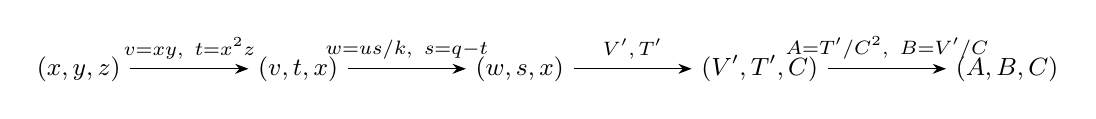
\begin{tikzpicture}[node distance=1.5cm, every node/.style={font=\small}, >=Stealth]
\node (xyz) {$(x,y,z)$};
\node (vtx) [right=of xyz] {$(v,t,x)$};
\node (wsx) [right=of vtx] {$(w,s,x)$};
\node (vpt) [right=of wsx] {$(V',T',C)$};
\node (abc) [right=of vpt] {$(A,B,C)$};
\draw[->] (xyz) -- node[above, font=\scriptsize]{$v{=}xy,\ t{=}x^2z$} (vtx);
\draw[->] (vtx) -- node[above, font=\scriptsize]{$w{=}us/k,\ s{=}q{-}t$} (wsx);
\draw[->] (wsx) -- node[above, font=\scriptsize]{$V',T'$} (vpt);
\draw[->] (vpt) -- node[above, font=\scriptsize]{$A{=}T'/C^2,\ B{=}V'/C$} (abc);
\end{tikzpicture}
\caption{Reduction chain of the skew product: the Jacobian determinant is the product of the determinants of the four steps (Lemma~\ref{lem:skew}), and the two-variable identity lives in the middle step, from $(v,t)$ to $(V',T')$ through the pair $(w,s)$.}
\label{fig:chain}
\end{figure}

\begin{lemma}[Skew-product determinant lemma, {\DD}, certified {\MV} with generic symbolic coefficients]\label{lem:skew}
For \emph{any} polynomials $a_1, b_1, c_1$ in $(v, t)$ with $c_1 \ne 0$, the map
$(a_1/x^2,\, b_1/x,\, x c_1)|_{v = xy,\, t = x^2 z}$ satisfies
\begin{equation}\label{eq:skew}
\detJ \cdot c_1^2 = -J_2, \qquad
J_2 = \det \frac{\partial (V', T')}{\partial (v, t)}, \quad V' = b_1 c_1, \; T' = a_1 c_1^2 .
\end{equation}
\end{lemma}
\begin{proof}
Write $C = x c_1$, $A = T'/C^2$ and $B = V'/C$, so that the map is $(A, B, C)$. By the chain rule through the variables $(v,t,x)$ and $(V',T',C)$,
$\partial(A,B,C)/\partial(x,y,z)$ is the product of three matrices. The matrix $\partial(A,B,C)/\partial(V',T',C)$ has rows $(0, C^{-2}, \ast)$, $(C^{-1}, 0, \ast)$, $(0,0,1)$, hence determinant $-C^{-3}$.
The matrix $\partial(V',T',C)/\partial(v,t,x)$ has rows $(V'_v, V'_t, 0)$, $(T'_v, T'_t, 0)$, $(\ast, \ast, c_1)$, hence determinant $c_1 J_2$. The matrix $\partial(v,t,x)/\partial(x,y,z)$ has rows $(y, x, 0)$, $(2xz, 0, x^2)$, $(1,0,0)$, hence determinant $x^3$.
The product is $-C^{-3}\, c_1 J_2\, x^3 = -J_2/c_1^2$ because $C^3 = x^3c_1^3$.
\end{proof}

For $F$ the reduced data \eqref{eq:reduced} give $J_2 = 2 c_1^2$ \MV: the Keller property is a \emph{two-variable} identity, and the third dimension only carries weights. The identity $J_2 = 2c_1^2$ and the determinant $-2$ were obtained independently of the three-variable expansion of Section~\ref{sec:valid}, which removes the dependence on a single route. Fibers are governed by a single cubic. With $w = u c_1 / 2$ and $\Phi(w) = w^2 - w^3$,
\begin{equation}\label{eq:fiber}
\Phi(w) = \tfrac14\left(w\, QR - P R^2\right) \quad \text{identically \MV},
\end{equation}
so preimages of $(A, B, C)$ correspond to roots of $4\Phi(w) - w BC + A C^2 = 0$; at the announced target this degenerates to $\Phi(w) = 0$ with roots $\{0, 0, 1\}$, matching the three
preimages' $w$-values $(1, 0, 0)$ \MV. Injectivity dies by \emph{non-properness}: a Keller map is a local diffeomorphism, so two sheets of preimages cannot merge at a finite point, where $\detJ$ would have to vanish; they merge only at infinity. This is the loophole that Pinchuk used in the real non-constant case and the modern form of the gap in Kraus' argument. The weight symmetry also explains why the three-dimensional map is a one-variable problem in disguise: the weight-zero invariants $v$ and $t$ and the single scale $x$ carry all the coordinates, the output invariants $V'$ and $T'$ are functions of $(v,t)$ alone, and the determinant of the whole map is the determinant of the two-variable map $(v,t) \mapsto (V',T')$ divided by $c_1^2$. The generating identity says that the first component carries no independent information: the map is generated by the pair $(b_1, c_1)$, which is the observation that the constructor of Section~\ref{sec:family} turns into a machine.

\section[The seed family: constructor, proof, instances and degree laws]{The seed family: constructor, proof, instances\\ and degree laws}\label{sec:family}

\subsection{The first constructor and its failure (EXP-003)}\label{sec:first}

The first attempt at a constructor identifies $c_1 = h(v) - t$ with $h(w) = p(w)/w$, sets $w = uc_1/k$ and takes $b_1 = k u\, h(u c_1/k) + m$ and $a_1 = u b_1/k - k^2\Phi(uc_1/k)/c_1^2$, which is polynomial because $\Phi$ starts at $w^2$.

\begin{proposition}[Unsolvability of the first constructor, {\MV}]\label{prop:first}
For a seed of degree $2$, $p = p_1 w + p_2 w^2$, polynomiality of the three components and a constant determinant force, besides the zero solution, exactly the branch $p_1 = k$, $p_2 = -3k/2$, $m = k^2/2$, with $\det JF = -k^3/4$; the announced map is the instance $k = 2$. For the seeds $p = w - 2w^3$ and $p = 8w - 12w^2 + 4w^3 - 5w^4$ the polynomiality conditions have no solution $(k, m)$.
\end{proposition}

The statement is an exact emptiness statement for a polynomial system over $\Q$, not a numerical failure. Its meaning is that the identification $c_1 = h(v) - t$ is a degree-two coincidence ($h$ is affine exactly when $\deg p = 2$) and not the general law. At degree two the announced map is, up to the scale $k$, the unique map of this shape, and its determinant $-k^3/4$ agrees with the value $-k\,p(1)^2$ of Theorem~\ref{thm:family} because $p(1) = -k/2$ on that branch. The failure analysis leads to the potential form below, in the reduced coordinates $(w, s)$ with $s = c_1$, where the fiber identity $\Phi(w) = (wV' - T')/k^2$ holds by construction instead of by coincidence.

\subsection{The constructor theorem and its proof}\label{sec:constructor}

\begin{theorem}[Constructor, {\DD}, certified on instances {\MV}]\label{thm:family}
Let $p(w) = \sum_{i=1}^{d} p_i w^i$ have degree $d$ and satisfy the admissibility conditions
\begin{equation}\label{eq:adm}
p(0) = 0, \qquad \int_0^1 p = 0, \qquad p(1) \ne 0, \qquad p'(1) \ne 2 p(1),
\end{equation}
let $k \ne 0$, $m = -k\,p(1)$, and let $q(v)$ be any polynomial with $q(0) = k$ and
$q'(0) = k\,(p(1) - p'(1))/(p'(1) - 2p(1))$, with arbitrary higher-order tail. Set
$\Phi(w) = \int_0^w p$, $s = c_1 = q(v) - t$, $w = u s / k$, and define
\begin{equation}\label{eq:potential}
V' = k^2 p(w) + m s, \qquad T' = w V' - k^2 \Phi(w), \qquad
b_1 = V'/s, \qquad a_1 = T'/s^2 .
\end{equation}
Then $a_1, b_1$ are polynomials in $(v, t)$, and
$F_{p, k, q} = (a_1 / x^2,\; b_1 / x,\; x c_1)$ is a polynomial Keller map of $\C^3$ with
\begin{equation}\label{eq:detfamily}
\det J F_{p,k,q} = -\frac{m^2}{k} = -k\,p(1)^2 \quad (\text{constant, for every admissible } (p,k,q)).
\end{equation}
Over a target $(A,B,C)$ with $C \neq 0$ the fiber is in bijection with the simple roots of the fiber polynomial
$W(w) = k^2\Phi(w) - w\,BC + AC^2$, which has degree $d+1$; for $(A,B,C)$ outside a proper closed subset the fiber has exactly $d+1$ points. A root $w$ of $W$ reconstructs its preimage by
\begin{equation}\label{eq:reconstruct}
s = \frac{BC - k^2 p(w)}{m}, \quad u = \frac{k w}{s}, \quad x = \frac{C}{s}, \quad v = u - 1,
\quad t = q(v) - s, \quad y = \frac{v}{x}, \quad z = \frac{t}{x^2}.
\end{equation}
The announced map \eqref{eq:F} is the instance $p = 2w - 3w^2$, $k = 2$, $q$ affine; at $d = 2$ this shape is rigid up to the scale $k$ \MV{} (Proposition~\ref{prop:first}).
\end{theorem}

\begin{proof}
\emph{Step 1: polynomiality in $(v,t)$.} Since $p(0) = 0$ and $\Phi(0) = \Phi'(0) = 0$, write $p(w) = w\,r(w)$ and $\Phi(w) = w^2\rho(w)$ with $r, \rho \in \Q[w]$. Because $w = us/k$ is a polynomial in $(v,t)$ divisible by $s$, $p(w)/s = (u/k)\,r(w)$ is a polynomial. Moreover $T' = k^2 w^2 r(w) + m w s - k^2 w^2\rho(w)$ and $w = us/k$ give
\begin{equation}\label{eq:closed}
b_1 = k\,u\,r(w) + m, \qquad a_1 = u^2\bigl(r(w) - \rho(w)\bigr) + \tfrac{m}{k}\,u,
\end{equation}
both polynomials in $(v,t)$. For the announced seed these closed forms reproduce, on $t = 0$, the polynomials $b_1 = v + 12v^2 + 9v^3$ and $a_1 = u(4v^2 + 3v^3)$ of Theorem~\ref{thm:structure}.

\emph{Step 2: polynomiality in $(x,y,z)$ and the admissibility conditions.} A monomial $v^i t^j$ of $a_1$ becomes $x^{i+2j-2}y^iz^j$ in $a_1/x^2$ and one of $b_1$ becomes $x^{i+2j-1}y^iz^j$ in $b_1/x$. Hence the map is polynomial exactly when $a_1$ has no monomial $1$ or $v$ and $b_1$ has no constant term. At the origin $s = q(0) = k$, $u = 1$, $w = 1$. Then $b_1(0,0) = k\,p(1) + m$ vanishes if and only if $m = -k\,p(1)$. With this value $V'(0,0) = k^2p(1) + mk = 0$, so $T'(0,0) = -k^2\Phi(1)$ and $a_1(0,0) = -\Phi(1)$, which vanishes if and only if $\int_0^1 p = 0$. Given these, $\partial_v a_1(0,0) = T'_v(0,0)/k^2$; the differential of $T'$ at the origin equals $k^2\bigl(p'(1) - p(1)\bigr)\,dw + m\,ds$ with $w_v = (k + q'(0))/k$ and $s_v = q'(0)$, so
\begin{equation}\label{eq:tv}
T'_v(0,0) = k\bigl[(p'(1) - p(1))\,k + q'(0)\,(p'(1) - 2p(1))\bigr],
\end{equation}
which vanishes if and only if $q'(0) = k\,(p(1) - p'(1))/(p'(1) - 2p(1))$. If $p'(1) = 2p(1)$ the condition would read $p(1)\,k = 0$, impossible since $p(1) \neq 0$ and $k \ne 0$: the fourth admissibility condition is necessary. The conditions are therefore equivalent to the polynomiality of the lifted map, and they are exactly the conditions at weights $0$ and $1$ at the origin. The third component $x c_1 = x(q(v) - t)$ is a polynomial.

\emph{Step 3: the determinant.} From $T' = wV' - k^2\Phi(w)$ one gets $dT' = (V' - k^2p(w))\,dw + w\,dV' = m s\,dw + w\,dV'$ because $V' - k^2p(w) = ms$, and $dV' = k^2p'(w)\,dw + m\,ds$. Therefore $dV'\wedge dT' = ms\,dV'\wedge dw = -m^2 s\,dw\wedge ds$. For the change of variables $(v,t)\mapsto(w,s)$, $s_v = q'$, $s_t = -1$, $w_v = (s + uq')/k$, $w_t = -u/k$, so $\partial(w,s)/\partial(v,t) = w_v s_t - w_t s_v = -s/k$. Hence $J_2 = (-m^2s)(-s/k) = m^2 s^2/k$, and Lemma~\ref{lem:skew} with $c_1 = s$ gives $\det J F_{p,k,q} = -J_2/c_1^2 = -m^2/k = -k\,p(1)^2$.

\emph{Step 4: the fiber and the reconstruction.} A point of $\C^3$ maps to $(A,B,C)$ if and only if $V' = BC$, $T' = AC^2$ and $C = xs$ (since $A = T'/C^2$, $B = V'/C$). Eliminating $T'$ by $T' = wV' - k^2\Phi(w)$ gives $W(w) = 0$. Differentiating, $W'(w) = k^2p(w) - BC$, so $s = (BC - k^2p(w))/m = -W'(w)/m$. If $C \neq 0$ then $x \neq 0$ and $s \neq 0$, so every preimage yields a root $w$ with $W'(w) = -ms \neq 0$: a simple root. Conversely a simple root $w$ defines $s \ne 0$ by \eqref{eq:reconstruct}, hence $u$, $x$, $v$, $t$, $y$, $z$; the pair $(v,t)$ satisfies $s = q(v) - t$ and $w = us/k$ by construction, so $V' = k^2p(w) + ms = BC$ and $T' = wBC - k^2\Phi(w) = AC^2$ (the root condition), and then $(a_1/x^2, b_1/x, xc_1) = (T'/(s^2x^2), V'/(sx), xs) = (A,B,C)$. Distinct roots give distinct preimages, since $w$ is a function of the preimage.

\emph{Step 5: the fiber degree.} $W$ has degree $d+1$ with leading coefficient $k^2p_d/(d+1) \neq 0$. For fixed $B$ and $C \neq 0$, $W_A(w) = g(w) + AC^2$ with $g(w) = k^2\Phi(w) - wBC$, and $W_A$ has a multiple root only if $g'(w) = k^2p(w) - BC = 0$ and $g(w) = -AC^2$. The polynomial $k^2 p - BC$ is nonzero, so it has finitely many roots, and only finitely many values of $A$ make $W_A$ non-squarefree. The discriminant of $W$ is therefore a nonzero polynomial in $(A,B,C)$, and off its zero set the fiber has exactly $d+1$ points.
\end{proof}

The three admissibility conditions are exactly the low-weight polynomiality constraints at the origin; the potential form makes $J_2 = m^2 s^2/k$ automatic, so \emph{the Keller property costs nothing}: this is the structural reason the conjecture is false in dimension $\ge 3$. The proof is machine-checked on instances (Table~\ref{tab:instances}): for each of them $J_2 = m^2c_1^2/k$, the three components are polynomial, the determinant is constant, the fiber polynomial is squarefree at a rational target, and the reconstruction \eqref{eq:reconstruct} is verified modulo the fiber polynomial.

\subsection{Instances and collision certificates}\label{sec:instances}

\begin{table}[t]\centering\small\setlength{\tabcolsep}{4pt}
\begin{tabular}{llrrrccc}
\toprule
Instance & Seed $p$ & $d$ & $k$ & Section tail & $\det$ & Component degrees & Fiber degree \\
\midrule
$F$ & $2w - 3w^{2}$ & 2 & 2 & affine & $-2$ & $(7,\,6,\,4)$ & 3 \\
$G_3$ & $w - 2w^{3}$ & 3 & 3 & affine & $-3$ & $(12,\,11,\,4)$ & 4 \\
$G_4$ & $8w - 12w^{2} + 4w^{3} - 5w^{4}$ & 4 & 14 & affine & $-350$ & $(17,\,16,\,4)$ & 5 \\
$G_5$ & $w - 3w^{5}$ & 5 & 5 & affine & $-20$ & $(22,\,21,\,4)$ & 6 \\
$F^{\mathrm{tail}}$ & $2w - 3w^{2}$ & 2 & 2 & $v^2$ & $-2$ & $(8,\,7,\,5)$ & 3 \\
\bottomrule
\end{tabular}

\caption{Instances of the constructor, read from the stored outputs of computations EXP-004 and EXP-008: the seed $p$ of degree $d$, the scale $k$, the section tail beyond degree one, the determinant $-k\,p(1)^2$, the total degrees of the three components and the generic fiber degree $d+1$. Instance $F$ is the announced map.}
\label{tab:instances}
\end{table}

\begin{theorem}[New explicit counterexamples, {\MV}]\label{thm:instances}
The five maps of Table~\ref{tab:instances} are non-injective polynomial Keller maps of $\C^3$ with the determinants and component degrees shown, each certified by the engineered rational collision of Table~\ref{tab:collisions}. Their generic fiber degrees are $3$, $4$, $5$, $6$ and $3$.
\end{theorem}

\begin{table}[t]\centering\footnotesize\setlength{\tabcolsep}{3pt}
\begin{tabular}{lcll}
\toprule
Instance & Target $(A,B,C)$ & First preimage $(x,y,z)$ & Second preimage $(x,y,z)$ \\
\midrule
$F$ & $(-16,\,-16,\,1)$ & $(-\tfrac{1}{6},\,8,\,432)$ & $(\tfrac{1}{8},\,-4,\,-288)$ \\
$G_3$ & $(-54,\,-54,\,1)$ & $(-\tfrac{1}{15},\,18,\,5130)$ & $(\tfrac{1}{24},\,-18,\,-10368)$ \\
$G_4$ & $(-6272,\,-6272,\,1)$ & $(-\tfrac{5}{378},\,\tfrac{448}{5},\,\tfrac{80099712}{125})$ & $(\tfrac{5}{672},\,-\tfrac{532}{5},\,-\tfrac{237890688}{125})$ \\
$G_5$ & $(-750,\,-750,\,1)$ & $(-\tfrac{1}{70},\,75,\,399000)$ & $(\tfrac{1}{160},\,-150,\,-3824000)$ \\
$F^{\mathrm{tail}}$ & $(-16,\,-16,\,1)$ & $(-\tfrac{1}{6},\,8,\,496)$ & $(\tfrac{1}{8},\,-4,\,-272)$ \\
\bottomrule
\end{tabular}

\caption{Engineered collisions: for each instance of Table~\ref{tab:instances} the target $(A,B,C)$ with $C = 1$ and two distinct rational preimages that both map to it, obtained by Algorithm~\ref{alg:collision} with prescribed fiber roots $w_1 = 1$ and $w_2 = 2$; all images are verified by exact substitution into the full components.}
\label{tab:collisions}
\end{table}

For the announced map the engineering reproduces the target $(-16,-16,1)$: with $k = 2$ and $k^2\Phi(w) = 4(w^2 - w^3)$ the linear system $V - T = 0$, $2V - T = -16$ gives $V = T = -16$, and $s_1 = (V - 4p(1))/2 = -6$ yields $x_1 = -\tfrac16$. The section-tail instance $F^{\mathrm{tail}}$ changes the component-degree pattern at fixed fiber degree and determinant: the family is strictly larger than the seed-only family. Every negative rational number is realized as a Keller determinant within the family, since $\det = -k\,p(1)^2$ scales linearly with $k$.

\begin{remark}[Characteristic $p$, {\MV}]\label{rem:charp}
The instance $G_3$ reduces modulo $\ell = 13$ and $\ell = 101$ to explicit non-injective Keller maps over $\mathbb{F}_\ell$ of total degree $12 < \ell$. All coefficients are $\ell$-integral, the determinant $-3$ is \numDetModThirteen{} modulo $13$ and \numDetModHundred{} modulo $101$, and the rational collision reduces to distinct points with a common image: modulo $13$, \ptModThirteenA{} and \ptModThirteenB{} both map to \ptModThirteenT{}; modulo $101$, \ptModHundredA{} and \ptModHundredB{} both map to \ptModHundredT{}. Unlike the classical example $x - x^p$, whose degree equals $p$, the degree sits strictly below the characteristic, as integer-model reductions lead one to expect; here it is certified explicitly.
\end{remark}

\subsection{Degree laws and the scope of the minimality claim}\label{sec:degrees}

\begin{figure}[t]\centering
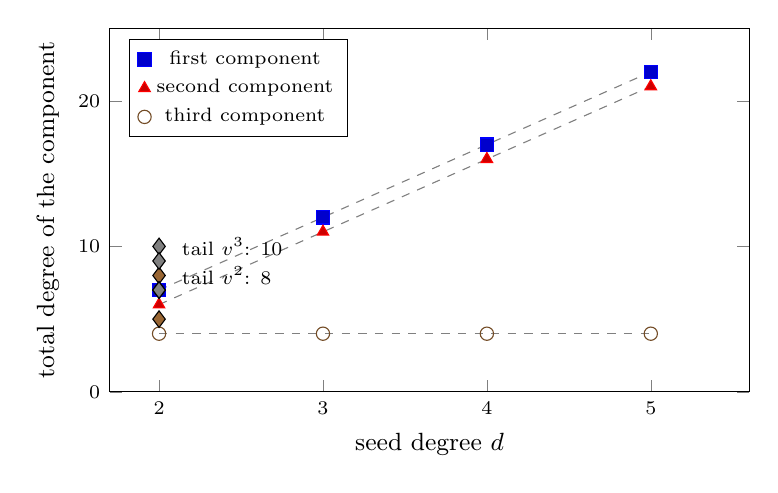
\begin{tikzpicture}
\begin{axis}[width=0.8\linewidth, height=6.2cm, xlabel={seed degree $d$}, ylabel={total degree of the component},
 xtick={2,3,4,5}, xmin=1.7, xmax=5.6, ymin=0, ymax=25, legend pos=north west, legend style={font=\scriptsize}, tick label style={font=\scriptsize}, label style={font=\small}]
\addplot+[only marks, mark=square*, mark size=2.4pt] coordinates {(2,7) (3,12) (4,17) (5,22)};
\addlegendentry{first component}
\addplot+[only marks, mark=triangle*, mark size=2.4pt] coordinates {(2,6) (3,11) (4,16) (5,21)};
\addlegendentry{second component}
\addplot+[only marks, mark=o, mark size=2.4pt] coordinates {(2,4) (3,4) (4,4) (5,4)};
\addlegendentry{third component}
\addplot[dashed, domain=2:5, samples=2, gray] {5*x-3};
\addplot[dashed, domain=2:5, samples=2, gray] {5*x-4};
\addplot[dashed, domain=2:5, samples=2, gray] {4};
\addplot+[only marks, mark=diamond*, mark size=3pt, black] coordinates {(2,8) (2,7) (2,5)};
\node[font=\scriptsize, anchor=west] at (axis cs:2.08,8) {tail $v^2$: $8$};
\addplot+[only marks, mark=diamond*, mark size=3pt, black] coordinates {(2,10) (2,9) (2,7)};
\node[font=\scriptsize, anchor=west] at (axis cs:2.08,10) {tail $v^3$: $10$};

\end{axis}
\end{tikzpicture}
\caption{Total degrees of the three components of the instances $F$, $G_3$, $G_4$, $G_5$ of Table~\ref{tab:instances} against the seed degree $d$ (markers, read from the stored output of EXP-008), with the law $5d-3$, $5d-4$, $4$ (dashed), and the degrees of the section-tail variants of $F$ (diamonds).}
\label{fig:degrees}
\end{figure}

\begin{theorem}[Degree law on four seeds, {\MV}]\label{thm:degrees}
For the four seeds of $F$, $G_3$, $G_4$ and $G_5$ (Table~\ref{tab:instances}) with affine sections, the component total degrees are exactly $(5d - 3,\, 5d - 4,\, 4)$ for $d = 2, 3, 4, 5$. At $d = 2$ the scale $k = 7$ gives the same degrees $(7,6,4)$, and the section tails $v^2$ and $v^3$ give $(8,7,5)$ and $(10,9,7)$, strictly larger in every component. A seed of degree $1$ is impossible: $p = p_1 w$ and $\int_0^1 p = p_1/2 = 0$ force $p = 0$, so the fiber degree in the family is at least $3$. Among the instances of Table~\ref{tab:instances} the minimal degree vector is $(7,6,4)$, attained at the announced map. Globally only Wang's theorem constrains $\C^3$; the existence of a counterexample of total degree $3$ to $6$ is open~\UU{} (no source in the literature read for this work settles it).
\end{theorem}

The theorem is a statement about the four seeds that were computed: the machine verification covers one seed per degree $d$, the scale $k = 7$ at $d = 2$ and the tails $v^2$, $v^3$ at $d = 2$ (Figure~\ref{fig:degrees}). It does not cover other seeds of the same degree, other scales at $d \ge 3$, or tails at $d \ge 3$.

\begin{conjecture}[Degree law and minimality in the family, {\CC}]\label{conj:degrees}
For every admissible seed of degree $d \ge 2$, every scale $k$ and every affine section, the component total degrees of $F_{p,k,q}$ are $(5d-3, 5d-4, 4)$; every nonzero tail strictly increases them; and consequently the minimal degree vector over the whole family is $(7,6,4)$, attained exactly at the announced map, up to the scale $k$.
\end{conjecture}

The evidence is the machine verification above and the structure of \eqref{eq:closed}: the leading monomials of the components arise from the top powers of $w$ in $r(w) - \rho(w)$ and $r(w)$, whose coefficients are multiples of the leading coefficient of the seed. A proof would show that no cancellation occurs among those top monomials for every seed, every scale and every tail; it is not carried out here, and the minimality of the announced map within the family is a conjecture until it is.

\section{The asymptotic variety: where sheets merge}\label{sec:asymptotic}

\begin{theorem}[Escape and the discriminant wall; part 1 {\DD}, certified {\MV} on $F$ and $G_3$ (EXP-007); part 2 {\DD}, with the plane samples {\MV} (EXP-145)]\label{thm:asymptotic}
Let $F$ be the announced map, $W(w) = 4(w^2 - w^3) - wBC + AC^2$ its fiber polynomial, $D$ the discriminant of $W$ in $w$ and
\begin{equation}\label{eq:sigma}
\Sigma(A,B,C) = 27A^2C^2 - 18ABC + 16A + B^3C - B^2, \qquad D = -16\,C^2\,\Sigma .
\end{equation}
\begin{enumerate}
\item In the potential form $W'(w) = k^2 p(w) - BC$ identically and the reconstruction scale is $s = -W'(w)/m$. Over $C \neq 0$ a root of $W$ reconstructs a finite preimage if and only if it is a simple root; a multiple root corresponds to a preimage that has escaped to infinity.
\item The asymptotic variety of $F$, the set of limits of $F(p_n)$ along sequences $p_n \to \infty$, is the surface $\{\Sigma = 0\}$. The plane $C = 0$ is not contained in it.
\end{enumerate}
\end{theorem}

Part 1 is Step 4 of the proof of Theorem~\ref{thm:family}, with the machine-verified identities $W' = k^2p - BC$ and $s = -W'/m$ for $F$ and $G_3$ (EXP-007), and the discriminant $D = -16C^2\Sigma$ computed by sympy \MV. Part 2 depends on the fibers over the plane $C = 0$, which Theorem~\ref{thm:cplane} gives; its proof is at the end of this section. In the chart $C = 1$ the factor $C^2$ of $D$ records the degeneration of the reconstruction at $C = 0$, where $x = C/s$ is no longer determined, and not an asymptotic locus.

\begin{theorem}[Fibers over the plane $C = 0$, {\DD}; the parametrization identity and \numPlaneTargets{} sampled targets {\MV}, EXP-145]\label{thm:cplane}
Since $F(0,y,z) = (z + 4y^2,\, y,\, 0)$, the fiber of $F$ over $(A,B,0)$ contains the flat-sheet point $(0, B, A - 4B^2)$. A preimage with $x \neq 0$ has $c_1 = 0$, hence $b_1 = 6 + 4v = Bx$ and $a_1 = (1+v)(2+v) = Ax^2$, which are equivalent to
\begin{equation}\label{eq:cplane}
x^2\,(B^2 - 16A) = 4, \qquad y = \frac{Bx - 6}{4x}, \qquad z = \frac{26 - 3Bx}{4x^2}.
\end{equation}
If $B^2 \neq 16A$ the fiber therefore has exactly three points, the flat-sheet point and the two points with $x = \pm 2/\sqrt{B^2 - 16A}$; if $B^2 = 16A$ it has the flat-sheet point only.
\end{theorem}

\begin{proof}
On $c_1 = 0$ one has $t = 2 - 3v$ and, from the formulas of Theorem~\ref{thm:structure}, $b_1 = 3(2-3v)u^2 + 9v^3 + 12v^2 + v = 6 + 4v$ and $a_1 = (v+1)\bigl((2-3v)u^2 + 3v^3 + 4v^2\bigr) = (1+v)(2+v)$. With $u = 1 + v$ the first equation gives $u = (Bx - 2)/4$ and the second becomes $Ax^2 = u(u+1) = (B^2x^2 - 4)/16$, which is the first relation of \eqref{eq:cplane}; $y = v/x$ and $z = t/x^2$ give the others.
\end{proof}

At $(A,B) = (-\tfrac14, 0)$ one has $B^2 - 16A = 4$, $x = \pm 1$, $y = \mp\tfrac32$ and $z = \tfrac{13}{2}$: the three announced points of Theorem~\ref{thm:valid}. A second instance is the target $(0,1,0)$, with $B^2 - 16A = 1$: the fiber contains $(0, 1, -4)$, $(2, -\tfrac12, \tfrac54)$ and $(-2, 1, 2)$, which all map to $(0,1,0)$ by direct substitution; computation EXP-145 solves this fiber and that of the announced target from their Gr\"obner bases and verifies the images exactly. It verifies symbolically that $F(0,y,z) = (z + 4y^2, y, 0)$ and that the points of \eqref{eq:cplane} map to $(A,B,0)$ on $x^2(B^2 - 16A) = 4$, and it finds \numPlaneThree{} sampled targets with $B^2 \neq 16A$ whose fibers have exactly three distinct points (\numPlaneNonreal{} of them with non-real points) and \numPlaneOne{} with $B^2 = 16A$ whose fibers have one point (Figure~\ref{fig:plane}).

\begin{proof}[Proof of Theorem~\ref{thm:asymptotic}, part 2]
\emph{Targets off the surface.} Let $t_0 = (A_0,B_0,C_0)$ with $\Sigma(t_0) \neq 0$. If $C_0 \neq 0$, $W_{t_0}$ has three simple roots, which depend continuously on the target; by Part 1 the preimages of every nearby target are the three reconstructions of Theorem~\ref{thm:family}, with $s = -W'(w)/m$ bounded away from zero, so they stay bounded. If $C_0 = 0$, then $B_0^2 \neq 16A_0$, and by Theorem~\ref{thm:cplane} the fiber over $t_0$ has three distinct points, at each of which $F$ is a local biholomorphism ($\detJ = -2$). Let $U_1, U_2, U_3$ be disjoint neighborhoods of these points mapped onto a common neighborhood $N$ of $t_0$. For $t \in N$ with $C \ne 0$ the three preimages in the $U_i$ are all the preimages, since there are at most three; for $t \in N$ with $C = 0$ the fiber has exactly three points by Theorem~\ref{thm:cplane}. So all preimages of targets in $N$ lie in $U_1 \cup U_2 \cup U_3$, and no sequence $p_n \to \infty$ has $F(p_n) \to t_0$.
\emph{Targets on the surface.} If $C_0 \neq 0$ and $\Sigma(t_0) = 0$, choose targets $t_n \to t_0$ off the surface; $W_{t_n}$ has simple roots $w_n$ converging to a multiple root $w_0$ of $W_{t_0}$, so $s_n = -W'_{t_n}(w_n)/m \to 0$ and the reconstructed preimage has $x_n = C_n/s_n \to \infty$ while $F(p_n) = t_n \to t_0$. If $C_0 = 0$ and $B_0^2 = 16A_0$, choose $(A_n, B_n) \to (A_0, B_0)$ with $B_n^2 - 16A_n \to 0$ and $\neq 0$: the points of Theorem~\ref{thm:cplane} with $x_n = 2/\sqrt{B_n^2 - 16A_n} \to \infty$ map to $(A_n, B_n, 0) \to t_0$.
\end{proof}

Verified end to end \MV: the target $(0, 1, 1)$ lies on the surface and its exact fiber is the single point $(2, -\tfrac12, \tfrac98)$ (a double root and a simple root of $W$: two sheets escaped; computation EXP-145 confirms a fiber ideal of quotient dimension $1$ at this target, so no irrational point is missed); the collision target $(-16, -16, 1)$ has $D = \numDcollision{} \neq 0$ and a full three-point rational fiber, whose third point is $(\tfrac{1}{24}, -28, -10656)$. Collisions are generic; escapes are of codimension one. Kraus' ``ramification at infinity'' is, for this family, the discriminant of a univariate polynomial. An enumeration that keeps only the rational solutions of the fiber system sees one point over a generic rational target $(A,B,0)$, because the two points of \eqref{eq:cplane} are irrational unless $B^2 - 16A$ is a rational square; computation EXP-145 recomputes the two rational targets of the enumeration of EXP-007 on the plane, finds three points over each with exactly one rational, and so supersedes, in part, the characterization of the asymptotic variety in EXP-007 (item 2, which includes the plane $C = 0$) and its statement that the plane is asymptotic with a single-point fiber (item 4); items 1, 3 and 5 of EXP-007 are not affected.

\section{Real fibers and the image of the map}\label{sec:real}

\begin{theorem}[Real census and image, {\DD}; the census {\MV} at the targets of Table~\ref{tab:census}; the emptiness over $\Gamma$ and the sampled fibers {\MV}, EXP-145]\label{thm:realcensus}
Over $\R$, the announced $F$ restricts to an orientation-reversing ($\det = -2$), non-proper, non-injective real Keller map. For real targets with $C \ne 0$ off the surface $\Sigma = 0$ the number of real preimages is $3$ (region $D > 0$, that is $\Sigma < 0$, which contains the collision targets) or $1$ (region $D < 0$); two independent exact routes (Sturm isolation of the fiber cubic plus reconstruction, versus Gr\"obner elimination) agree at all sampled targets. The image of $F$ is the complement of the curve
\begin{equation}\label{eq:gamma}
\Gamma = \Bigl\{\bigl(\tfrac{4}{27\,c^2},\ \tfrac{4}{3c},\ c\bigr) : c \neq 0\Bigr\},
\end{equation}
over $\C$ and, with $c$ real, over $\R$: $F$ is not surjective, and every other real target has a real preimage. Over $C = 0$ the fiber has three real points if $B^2 > 16A$ and one real point if $B^2 \le 16A$ (Theorem~\ref{thm:cplane}).
\end{theorem}

\begin{proof}
For $C \neq 0$ the fiber is in bijection with the simple roots of $W$ (Theorem~\ref{thm:family}), and a real target gives a cubic $W$ with real coefficients and leading coefficient $-4$. If $D > 0$ it has three distinct real roots; if $D < 0$ it has one real root and two complex roots, all simple; if $D = 0$ it has a double root and a simple root, both real, or a triple root. A triple root occurs exactly when $W'' = -24w + 8$ and $W'$ vanish together with $W$ at $w = \tfrac13$, that is when $BC = \tfrac43$ and $AC^2 = \tfrac{4}{27}$: the curve $\Gamma$. In that case $W = -4(w - \tfrac13)^3$ has no simple root and the fiber is empty. In every other case with $C \ne 0$ a simple real root exists. Over $\C$ the same argument holds: a cubic with constant leading coefficient $-4$ has no simple root exactly when it equals $-4(w - r)^3$, and the coefficient of $w$ and the constant term of $W$ then force $r = \tfrac13$ and the target to lie on $\Gamma$, so the image of $F$ is $\C^3 \setminus \Gamma$ over $\C$ as well. Over $C = 0$ the flat-sheet point $(0, B, A - 4B^2)$ is real and Theorem~\ref{thm:cplane} gives the count.
\end{proof}

\begin{table}[t]\centering\small
\begin{tabular}{lcccc}
\toprule
Target $(A,B,C)$ & Sign of $D$ & Real roots of $W$ & Real preimages (Gr\"obner) & Escaping roots \\
\midrule
$(-16,\,-16,\,1)$ & $+$ & 3 & 3 & 0 \\
$(10,\,0,\,1)$ & $-$ & 1 & 1 & 0 \\
$(0,\,5,\,1)$ & $-$ & 1 & 1 & 0 \\
$(-3,\,2,\,-1)$ & $-$ & 1 & 1 & 0 \\
$(\tfrac{1}{2},\,-\tfrac{1}{3},\,2)$ & $-$ & 1 & 1 & 0 \\
$(-5,\,7,\,3)$ & $-$ & 1 & 1 & 0 \\
\midrule
$(0,\,1,\,1)$ & $0$ & n/a & 1 (rational fiber) & n/a \\
$(-\tfrac14,\,0,\,0)$ & plane $C=0$ & n/a & 3 (Gr\"obner fiber) & n/a \\
\bottomrule
\end{tabular}

\caption{Real census of $F$ at the sampled targets, read from the stored outputs of EXP-011 (rows above the rule), EXP-007 and EXP-001: the sign of the discriminant $D$, the number of real roots of $W$ (Sturm route), the number of real points of the exact fiber (Gr\"obner route) and the number of escaping roots. The two routes agree at every target.}
\label{tab:census}
\end{table}

The counts $\numCensusThree$ target with three real preimages and $\numCensusOne$ with one occur among the six sampled targets of Table~\ref{tab:census}, so both regions are inhabited. A grid of \numGrid{} rational targets (three values for each of $A$ and $B$ and four for $C$) contains no target with an empty real fiber: for the \numGridNoPlane{} targets with $C \neq 0$ the census is computed, and for the \numGridPlane{} targets on $C = 0$ the explicit flat-sheet point is real. The grid does not meet the curve $\Gamma$, so it could not show the gap in the image; the image statement of Theorem~\ref{thm:realcensus} is the derivation above, certified by computation EXP-145 in three ways. The lexicographic Gr\"obner basis of the fiber ideal over $\Gamma(c)$ with $c$ inverted is $[1]$, so no point of $\C^3$ maps to $\Gamma$; the same construction with $\tfrac{5}{27}$ in place of $\tfrac{4}{27}$ does not give $[1]$, which excludes an artifact of the construction; and at \numImgTargets{} sampled targets with $C \neq 0$ off $\Gamma$ (\numImgRandom{} random, \numImgSigma{} on the surface $\Sigma = 0$ and \numImgNear{} within $10^{-3}$ of $\Gamma$ in each coordinate) the fiber ideal is proper, its quotient dimension equals the number of simple roots of $W$, and a real preimage exists. The reconstruction identity is exact modulo $W$. That every target off $\Gamma$ with $C \neq 0$ has a preimage is the simple-root argument, with the samples as evidence and not as a proof. Computation EXP-145 supersedes the surjectivity statements of EXP-011 (items 3 and 4) and the readings of the plane $C = 0$ in EXP-007 (items 2 and 4), where they disagree with it. The constant-Jacobian \emph{real} statement in dimension three falls with the same example; Pinchuk's planar counterexample \cite{Pinchuk1994} concerned the non-constant case.

\begin{figure}[t]\centering
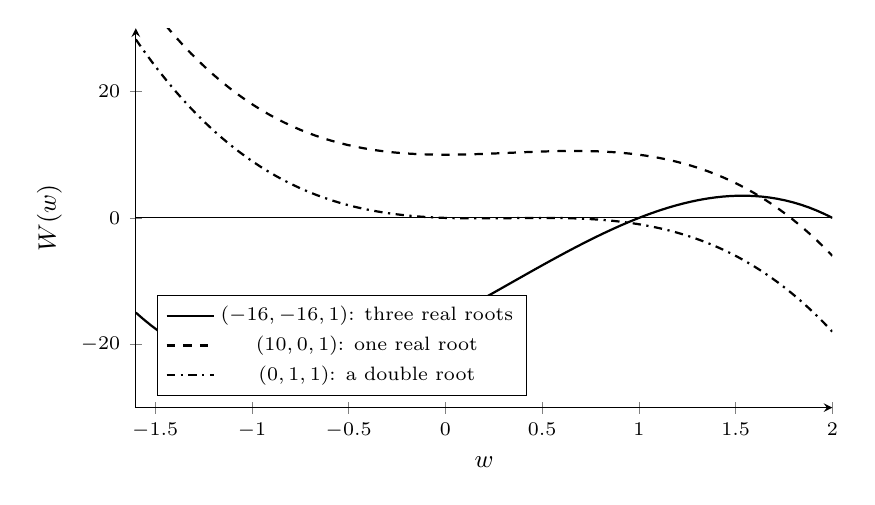
\begin{tikzpicture}
\begin{axis}[width=0.86\linewidth, height=6.4cm, xlabel={$w$}, ylabel={$W(w)$}, xmin=-1.6, xmax=2.0, ymin=-30, ymax=30,
 legend pos=south west, legend style={font=\scriptsize}, tick label style={font=\scriptsize}, label style={font=\small}, axis lines=left]
\addplot[thick, solid, domain=-1.6:2.0, samples=90] {4*(x^2-x^3) - x*(-16.0)*(1.0) + (-16.0)*(1.0)^2};
\addlegendentry{$(-16,-16,1)$: three real roots}
\addplot[thick, dashed, domain=-1.6:2.0, samples=90] {4*(x^2-x^3) - x*(0.0)*(1.0) + (10.0)*(1.0)^2};
\addlegendentry{$(10,0,1)$: one real root}
\addplot[thick, dashdotted, domain=-1.6:2.0, samples=90] {4*(x^2-x^3) - x*(1)*(1) + (0)*(1)^2};
\addlegendentry{$(0,1,1)$: a double root}
\addplot[black, forget plot, domain=-1.6:2.0, samples=2] {0};

\end{axis}
\end{tikzpicture}
\caption{The fiber polynomial $W(w) = 4(w^2 - w^3) - wBC + AC^2$ of the announced map at three targets of Table~\ref{tab:census}: three real roots (solid), one real root (dashed) and, at $(0,1,1)$ on the surface $\Sigma = 0$, a double root at $w = \tfrac12$ (dash-dotted), which is the escape of two sheets.}
\label{fig:fiber}
\end{figure}

\begin{figure}[t]\centering
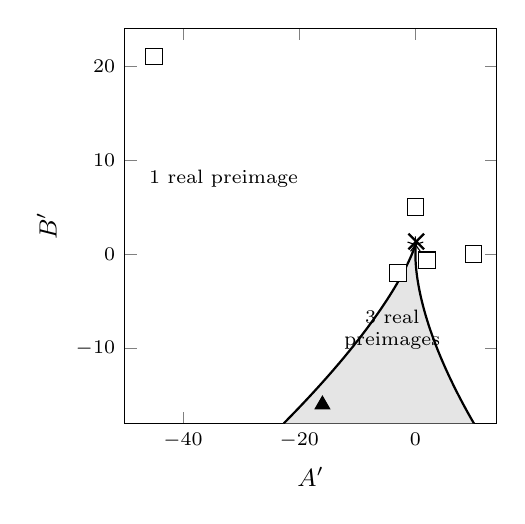
\begin{tikzpicture}\begin{axis}[width=0.52\linewidth, height=6.6cm, xlabel={$A'$}, ylabel={$B'$},
  xmin=-50, xmax=14, ymin=-18, ymax=24,
  tick label style={font=\scriptsize}, label style={font=\small}, clip=true]
\addplot[fill=black!10, draw=none] coordinates {(-22.65611,-18.00000) (-22.41859,-17.85157) (-22.18270,-17.70371) (-21.94845,-17.55642) (-21.71583,-17.40970) (-21.48482,-17.26356) (-21.25544,-17.11799) (-21.02766,-16.97299) (-20.80148,-16.82856) (-20.57690,-16.68470) (-20.35391,-16.54142) (-20.13252,-16.39871) (-19.91270,-16.25657) (-19.69446,-16.11500) (-19.47778,-15.97400) (-19.26268,-15.83358) (-19.04913,-15.69373) (-18.83713,-15.55445) (-18.62668,-15.41574) (-18.41778,-15.27760) (-18.21041,-15.14004) (-18.00457,-15.00305) (-17.80026,-14.86663) (-17.59747,-14.73078) (-17.39619,-14.59550) (-17.19642,-14.46080) (-16.99815,-14.32667) (-16.80139,-14.19311) (-16.60611,-14.06012) (-16.41232,-13.92770) (-16.22001,-13.79586) (-16.02917,-13.66459) (-15.83981,-13.53389) (-15.65191,-13.40376) (-15.46547,-13.27420) (-15.28048,-13.14522) (-15.09693,-13.01681) (-14.91483,-12.88897) (-14.73417,-12.76170) (-14.55493,-12.63500) (-14.37712,-12.50888) (-14.20073,-12.38333) (-14.02576,-12.25835) (-13.85219,-12.13394) (-13.68002,-12.01010) (-13.50926,-11.88684) (-13.33988,-11.76414) (-13.17189,-11.64202) (-13.00528,-11.52048) (-12.84004,-11.39950) (-12.67617,-11.27910) (-12.51367,-11.15926) (-12.35252,-11.04000) (-12.19273,-10.92131) (-12.03428,-10.80320) (-11.87718,-10.68565) (-11.72140,-10.56868) (-11.56696,-10.45228) (-11.41385,-10.33645) (-11.26205,-10.22120) (-11.11157,-10.10651) (-10.96239,-9.99240) (-10.81452,-9.87886) (-10.66794,-9.76589) (-10.52265,-9.65349) (-10.37865,-9.54167) (-10.23593,-9.43042) (-10.09448,-9.31974) (-9.95430,-9.20963) (-9.81538,-9.10009) (-9.67773,-8.99113) (-9.54132,-8.88273) (-9.40616,-8.77491) (-9.27224,-8.66767) (-9.13955,-8.56099) (-9.00810,-8.45489) (-8.87786,-8.34935) (-8.74885,-8.24439) (-8.62105,-8.14000) (-8.49445,-8.03619) (-8.36906,-7.93294) (-8.24487,-7.83027) (-8.12186,-7.72817) (-8.00004,-7.62664) (-7.87940,-7.52568) (-7.75993,-7.42530) (-7.64163,-7.32549) (-7.52449,-7.22625) (-7.40851,-7.12758) (-7.29368,-7.02948) (-7.17999,-6.93196) (-7.06745,-6.83500) (-6.95604,-6.73862) (-6.84576,-6.64281) (-6.73660,-6.54758) (-6.62856,-6.45291) (-6.52163,-6.35882) (-6.41581,-6.26530) (-6.31109,-6.17235) (-6.20746,-6.07997) (-6.10493,-5.98817) (-6.00348,-5.89694) (-5.90311,-5.80628) (-5.80381,-5.71619) (-5.70558,-5.62667) (-5.60841,-5.53773) (-5.51229,-5.44935) (-5.41723,-5.36155) (-5.32321,-5.27432) (-5.23023,-5.18767) (-5.13829,-5.10158) (-5.04737,-5.01607) (-4.95748,-4.93113) (-4.86861,-4.84676) (-4.78074,-4.76296) (-4.69388,-4.67974) (-4.60803,-4.59709) (-4.52316,-4.51500) (-4.43929,-4.43350) (-4.35640,-4.35256) (-4.27449,-4.27219) (-4.19355,-4.19240) (-4.11358,-4.11318) (-4.03457,-4.03453) (-3.95651,-3.95645) (-3.87941,-3.87895) (-3.80325,-3.80202) (-3.72803,-3.72566) (-3.65374,-3.64987) (-3.58038,-3.57465) (-3.50794,-3.50001) (-3.43642,-3.42593) (-3.36581,-3.35243) (-3.29611,-3.27950) (-3.22731,-3.20715) (-3.15940,-3.13536) (-3.09237,-3.06415) (-3.02624,-2.99351) (-2.96098,-2.92344) (-2.89659,-2.85394) (-2.83307,-2.78502) (-2.77041,-2.71666) (-2.70860,-2.64888) (-2.64764,-2.58167) (-2.58753,-2.51504) (-2.52826,-2.44897) (-2.46982,-2.38348) (-2.41221,-2.31856) (-2.35541,-2.25421) (-2.29944,-2.19043) (-2.24427,-2.12722) (-2.18991,-2.06459) (-2.13635,-2.00253) (-2.08359,-1.94104) (-2.03161,-1.88012) (-1.98041,-1.81978) (-1.93000,-1.76001) (-1.88035,-1.70080) (-1.83147,-1.64218) (-1.78335,-1.58412) (-1.73598,-1.52663) (-1.68936,-1.46972) (-1.64349,-1.41338) (-1.59836,-1.35761) (-1.55395,-1.30241) (-1.51028,-1.24779) (-1.46732,-1.19373) (-1.42508,-1.14025) (-1.38355,-1.08734) (-1.34273,-1.03501) (-1.30260,-0.98324) (-1.26317,-0.93205) (-1.22442,-0.88143) (-1.18636,-0.83138) (-1.14898,-0.78190) (-1.11226,-0.73299) (-1.07621,-0.68466) (-1.04082,-0.63690) (-1.00608,-0.58971) (-0.97200,-0.54309) (-0.93855,-0.49705) (-0.90575,-0.45157) (-0.87357,-0.40667) (-0.84202,-0.36234) (-0.81109,-0.31859) (-0.78078,-0.27540) (-0.75108,-0.23279) (-0.72198,-0.19075) (-0.69348,-0.14928) (-0.66557,-0.10838) (-0.63825,-0.06805) (-0.61151,-0.02830) (-0.58535,0.01088) (-0.55975,0.04949) (-0.53472,0.08753) (-0.51026,0.12499) (-0.48634,0.16189) (-0.46297,0.19821) (-0.44015,0.23396) (-0.41786,0.26914) (-0.39610,0.30374) (-0.37487,0.33777) (-0.35416,0.37124) (-0.33397,0.40413) (-0.31428,0.43644) (-0.29510,0.46819) (-0.27641,0.49936) (-0.25822,0.52996) (-0.24051,0.55999) (-0.22329,0.58945) (-0.20654,0.61834) (-0.19026,0.64665) (-0.17444,0.67439) (-0.15908,0.70156) (-0.14418,0.72816) (-0.12972,0.75418) (-0.11571,0.77964) (-0.10213,0.80452) (-0.08898,0.82883) (-0.07626,0.85257) (-0.06396,0.87573) (-0.05207,0.89833) (-0.04059,0.92035) (-0.02951,0.94180) (-0.01883,0.96268) (-0.00855,0.98298) (0.00136,1.00272) (0.01088,1.02188) (0.02002,1.04047) (0.02880,1.05848) (0.03721,1.07593) (0.04527,1.09280) (0.05297,1.10911) (0.06033,1.12484) (0.06734,1.13999) (0.07402,1.15458) (0.08037,1.16859) (0.08639,1.18203) (0.09209,1.19490) (0.09748,1.20720) (0.10257,1.21893) (0.10735,1.23008) (0.11183,1.24066) (0.11602,1.25067) (0.11993,1.26011) (0.12355,1.26898) (0.12691,1.27727) (0.12999,1.28499) (0.13281,1.29214) (0.13537,1.29872) (0.13768,1.30473) (0.13975,1.31016) (0.14157,1.31502) (0.14316,1.31931) (0.14451,1.32303) (0.14565,1.32618) (0.14656,1.32875) (0.14726,1.33075) (0.14776,1.33218) (0.14805,1.33304) (0.14815,1.33333) (0.14805,1.33304) (0.14777,1.33218) (0.14731,1.33075) (0.14668,1.32875) (0.14588,1.32618) (0.14492,1.32303) (0.14379,1.31931) (0.14252,1.31502) (0.14110,1.31016) (0.13954,1.30473) (0.13785,1.29872) (0.13603,1.29214) (0.13408,1.28499) (0.13202,1.27727) (0.12984,1.26898) (0.12755,1.26011) (0.12517,1.25067) (0.12269,1.24066) (0.12012,1.23008) (0.11746,1.21893) (0.11473,1.20720) (0.11192,1.19490) (0.10904,1.18203) (0.10610,1.16859) (0.10311,1.15458) (0.10006,1.13999) (0.09697,1.12484) (0.09384,1.10911) (0.09067,1.09280) (0.08748,1.07593) (0.08426,1.05848) (0.08103,1.04047) (0.07778,1.02188) (0.07453,1.00272) (0.07127,0.98298) (0.06802,0.96268) (0.06479,0.94180) (0.06156,0.92035) (0.05836,0.89833) (0.05519,0.87573) (0.05205,0.85257) (0.04894,0.82883) (0.04588,0.80452) (0.04287,0.77964) (0.03992,0.75418) (0.03703,0.72816) (0.03420,0.70156) (0.03144,0.67439) (0.02876,0.64665) (0.02617,0.61834) (0.02366,0.58945) (0.02125,0.55999) (0.01894,0.52996) (0.01673,0.49936) (0.01463,0.46819) (0.01265,0.43644) (0.01079,0.40413) (0.00906,0.37124) (0.00746,0.33777) (0.00601,0.30374) (0.00469,0.26914) (0.00353,0.23396) (0.00252,0.19821) (0.00167,0.16189) (0.00099,0.12499) (0.00048,0.08753) (0.00015,0.04949) (0.00001,0.01088) (0.00005,-0.02830) (0.00029,-0.06805) (0.00072,-0.10838) (0.00137,-0.14928) (0.00222,-0.19075) (0.00329,-0.23279) (0.00459,-0.27540) (0.00611,-0.31859) (0.00787,-0.36234) (0.00986,-0.40667) (0.01210,-0.45157) (0.01460,-0.49705) (0.01734,-0.54309) (0.02035,-0.58971) (0.02363,-0.63690) (0.02718,-0.68466) (0.03100,-0.73299) (0.03512,-0.78190) (0.03952,-0.83138) (0.04421,-0.88143) (0.04921,-0.93205) (0.05452,-0.98324) (0.06013,-1.03501) (0.06606,-1.08734) (0.07232,-1.14025) (0.07891,-1.19373) (0.08583,-1.24779) (0.09308,-1.30241) (0.10069,-1.35761) (0.10865,-1.41338) (0.11696,-1.46972) (0.12563,-1.52663) (0.13468,-1.58412) (0.14409,-1.64218) (0.15389,-1.70080) (0.16407,-1.76001) (0.17464,-1.81978) (0.18560,-1.88012) (0.19697,-1.94104) (0.20874,-2.00253) (0.22093,-2.06459) (0.23353,-2.12722) (0.24656,-2.19043) (0.26002,-2.25421) (0.27391,-2.31856) (0.28824,-2.38348) (0.30302,-2.44897) (0.31825,-2.51504) (0.33394,-2.58167) (0.35009,-2.64888) (0.36671,-2.71666) (0.38380,-2.78502) (0.40137,-2.85394) (0.41943,-2.92344) (0.43797,-2.99351) (0.45702,-3.06415) (0.47656,-3.13536) (0.49662,-3.20715) (0.51718,-3.27950) (0.53827,-3.35243) (0.55988,-3.42593) (0.58201,-3.50001) (0.60469,-3.57465) (0.62790,-3.64987) (0.65167,-3.72566) (0.67598,-3.80202) (0.70085,-3.87895) (0.72628,-3.95645) (0.75229,-4.03453) (0.77887,-4.11318) (0.80602,-4.19240) (0.83377,-4.27219) (0.86210,-4.35256) (0.89103,-4.43350) (0.92057,-4.51500) (0.95071,-4.59709) (0.98147,-4.67974) (1.01284,-4.76296) (1.04484,-4.84676) (1.07747,-4.93113) (1.11074,-5.01607) (1.14464,-5.10158) (1.17920,-5.18767) (1.21440,-5.27432) (1.25027,-5.36155) (1.28680,-5.44935) (1.32400,-5.53773) (1.36187,-5.62667) (1.40042,-5.71619) (1.43966,-5.80628) (1.47959,-5.89694) (1.52022,-5.98817) (1.56155,-6.07997) (1.60360,-6.17235) (1.64635,-6.26530) (1.68982,-6.35882) (1.73402,-6.45291) (1.77895,-6.54758) (1.82462,-6.64281) (1.87103,-6.73862) (1.91818,-6.83500) (1.96609,-6.93196) (2.01476,-7.02948) (2.06419,-7.12758) (2.11440,-7.22625) (2.16538,-7.32549) (2.21713,-7.42530) (2.26968,-7.52568) (2.32302,-7.62664) (2.37715,-7.72817) (2.43209,-7.83027) (2.48784,-7.93294) (2.54440,-8.03619) (2.60179,-8.14000) (2.66000,-8.24439) (2.71904,-8.34935) (2.77891,-8.45489) (2.83963,-8.56099) (2.90120,-8.66767) (2.96362,-8.77491) (3.02690,-8.88273) (3.09105,-8.99113) (3.15606,-9.10009) (3.22196,-9.20963) (3.28873,-9.31974) (3.35639,-9.43042) (3.42494,-9.54167) (3.49440,-9.65349) (3.56475,-9.76589) (3.63602,-9.87886) (3.70820,-9.99240) (3.78130,-10.10651) (3.85533,-10.22120) (3.93029,-10.33645) (4.00618,-10.45228) (4.08302,-10.56868) (4.16081,-10.68565) (4.23956,-10.80320) (4.31926,-10.92131) (4.39993,-11.04000) (4.48157,-11.15926) (4.56418,-11.27910) (4.64778,-11.39950) (4.73237,-11.52048) (4.81794,-11.64202) (4.90452,-11.76414) (4.99211,-11.88684) (5.08070,-12.01010) (5.17031,-12.13394) (5.26093,-12.25835) (5.35259,-12.38333) (5.44528,-12.50888) (5.53901,-12.63500) (5.63378,-12.76170) (5.72960,-12.88897) (5.82647,-13.01681) (5.92440,-13.14522) (6.02340,-13.27420) (6.12348,-13.40376) (6.22462,-13.53389) (6.32686,-13.66459) (6.43018,-13.79586) (6.53459,-13.92770) (6.64010,-14.06012) (6.74672,-14.19311) (6.85445,-14.32667) (6.96329,-14.46080) (7.07326,-14.59550) (7.18436,-14.73078) (7.29658,-14.86663) (7.40995,-15.00305) (7.52446,-15.14004) (7.64012,-15.27760) (7.75693,-15.41574) (7.87491,-15.55445) (7.99405,-15.69373) (8.11436,-15.83358) (8.23585,-15.97400) (8.35853,-16.11500) (8.48239,-16.25657) (8.60745,-16.39871) (8.73371,-16.54142) (8.86117,-16.68470) (8.98985,-16.82856) (9.11974,-16.97299) (9.25085,-17.11799) (9.38319,-17.26356) (9.51677,-17.40970) (9.65158,-17.55642) (9.78764,-17.70371) (9.92495,-17.85157) (10.06351,-18.00000)} -- cycle;
\addplot[thick, black] coordinates {(0.14815,1.33333) (0.14805,1.33304) (0.14777,1.33218) (0.14731,1.33075) (0.14668,1.32875) (0.14588,1.32618) (0.14492,1.32303) (0.14379,1.31931) (0.14252,1.31502) (0.14110,1.31016) (0.13954,1.30473) (0.13785,1.29872) (0.13603,1.29214) (0.13408,1.28499) (0.13202,1.27727) (0.12984,1.26898) (0.12755,1.26011) (0.12517,1.25067) (0.12269,1.24066) (0.12012,1.23008) (0.11746,1.21893) (0.11473,1.20720) (0.11192,1.19490) (0.10904,1.18203) (0.10610,1.16859) (0.10311,1.15458) (0.10006,1.13999) (0.09697,1.12484) (0.09384,1.10911) (0.09067,1.09280) (0.08748,1.07593) (0.08426,1.05848) (0.08103,1.04047) (0.07778,1.02188) (0.07453,1.00272) (0.07127,0.98298) (0.06802,0.96268) (0.06479,0.94180) (0.06156,0.92035) (0.05836,0.89833) (0.05519,0.87573) (0.05205,0.85257) (0.04894,0.82883) (0.04588,0.80452) (0.04287,0.77964) (0.03992,0.75418) (0.03703,0.72816) (0.03420,0.70156) (0.03144,0.67439) (0.02876,0.64665) (0.02617,0.61834) (0.02366,0.58945) (0.02125,0.55999) (0.01894,0.52996) (0.01673,0.49936) (0.01463,0.46819) (0.01265,0.43644) (0.01079,0.40413) (0.00906,0.37124) (0.00746,0.33777) (0.00601,0.30374) (0.00469,0.26914) (0.00353,0.23396) (0.00252,0.19821) (0.00167,0.16189) (0.00099,0.12499) (0.00048,0.08753) (0.00015,0.04949) (0.00001,0.01088) (0.00005,-0.02830) (0.00029,-0.06805) (0.00072,-0.10838) (0.00137,-0.14928) (0.00222,-0.19075) (0.00329,-0.23279) (0.00459,-0.27540) (0.00611,-0.31859) (0.00787,-0.36234) (0.00986,-0.40667) (0.01210,-0.45157) (0.01460,-0.49705) (0.01734,-0.54309) (0.02035,-0.58971) (0.02363,-0.63690) (0.02718,-0.68466) (0.03100,-0.73299) (0.03512,-0.78190) (0.03952,-0.83138) (0.04421,-0.88143) (0.04921,-0.93205) (0.05452,-0.98324) (0.06013,-1.03501) (0.06606,-1.08734) (0.07232,-1.14025) (0.07891,-1.19373) (0.08583,-1.24779) (0.09308,-1.30241) (0.10069,-1.35761) (0.10865,-1.41338) (0.11696,-1.46972) (0.12563,-1.52663) (0.13468,-1.58412) (0.14409,-1.64218) (0.15389,-1.70080) (0.16407,-1.76001) (0.17464,-1.81978) (0.18560,-1.88012) (0.19697,-1.94104) (0.20874,-2.00253) (0.22093,-2.06459) (0.23353,-2.12722) (0.24656,-2.19043) (0.26002,-2.25421) (0.27391,-2.31856) (0.28824,-2.38348) (0.30302,-2.44897) (0.31825,-2.51504) (0.33394,-2.58167) (0.35009,-2.64888) (0.36671,-2.71666) (0.38380,-2.78502) (0.40137,-2.85394) (0.41943,-2.92344) (0.43797,-2.99351) (0.45702,-3.06415) (0.47656,-3.13536) (0.49662,-3.20715) (0.51718,-3.27950) (0.53827,-3.35243) (0.55988,-3.42593) (0.58201,-3.50001) (0.60469,-3.57465) (0.62790,-3.64987) (0.65167,-3.72566) (0.67598,-3.80202) (0.70085,-3.87895) (0.72628,-3.95645) (0.75229,-4.03453) (0.77887,-4.11318) (0.80602,-4.19240) (0.83377,-4.27219) (0.86210,-4.35256) (0.89103,-4.43350) (0.92057,-4.51500) (0.95071,-4.59709) (0.98147,-4.67974) (1.01284,-4.76296) (1.04484,-4.84676) (1.07747,-4.93113) (1.11074,-5.01607) (1.14464,-5.10158) (1.17920,-5.18767) (1.21440,-5.27432) (1.25027,-5.36155) (1.28680,-5.44935) (1.32400,-5.53773) (1.36187,-5.62667) (1.40042,-5.71619) (1.43966,-5.80628) (1.47959,-5.89694) (1.52022,-5.98817) (1.56155,-6.07997) (1.60360,-6.17235) (1.64635,-6.26530) (1.68982,-6.35882) (1.73402,-6.45291) (1.77895,-6.54758) (1.82462,-6.64281) (1.87103,-6.73862) (1.91818,-6.83500) (1.96609,-6.93196) (2.01476,-7.02948) (2.06419,-7.12758) (2.11440,-7.22625) (2.16538,-7.32549) (2.21713,-7.42530) (2.26968,-7.52568) (2.32302,-7.62664) (2.37715,-7.72817) (2.43209,-7.83027) (2.48784,-7.93294) (2.54440,-8.03619) (2.60179,-8.14000) (2.66000,-8.24439) (2.71904,-8.34935) (2.77891,-8.45489) (2.83963,-8.56099) (2.90120,-8.66767) (2.96362,-8.77491) (3.02690,-8.88273) (3.09105,-8.99113) (3.15606,-9.10009) (3.22196,-9.20963) (3.28873,-9.31974) (3.35639,-9.43042) (3.42494,-9.54167) (3.49440,-9.65349) (3.56475,-9.76589) (3.63602,-9.87886) (3.70820,-9.99240) (3.78130,-10.10651) (3.85533,-10.22120) (3.93029,-10.33645) (4.00618,-10.45228) (4.08302,-10.56868) (4.16081,-10.68565) (4.23956,-10.80320) (4.31926,-10.92131) (4.39993,-11.04000) (4.48157,-11.15926) (4.56418,-11.27910) (4.64778,-11.39950) (4.73237,-11.52048) (4.81794,-11.64202) (4.90452,-11.76414) (4.99211,-11.88684) (5.08070,-12.01010) (5.17031,-12.13394) (5.26093,-12.25835) (5.35259,-12.38333) (5.44528,-12.50888) (5.53901,-12.63500) (5.63378,-12.76170) (5.72960,-12.88897) (5.82647,-13.01681) (5.92440,-13.14522) (6.02340,-13.27420) (6.12348,-13.40376) (6.22462,-13.53389) (6.32686,-13.66459) (6.43018,-13.79586) (6.53459,-13.92770) (6.64010,-14.06012) (6.74672,-14.19311) (6.85445,-14.32667) (6.96329,-14.46080) (7.07326,-14.59550) (7.18436,-14.73078) (7.29658,-14.86663) (7.40995,-15.00305) (7.52446,-15.14004) (7.64012,-15.27760) (7.75693,-15.41574) (7.87491,-15.55445) (7.99405,-15.69373) (8.11436,-15.83358) (8.23585,-15.97400) (8.35853,-16.11500) (8.48239,-16.25657) (8.60745,-16.39871) (8.73371,-16.54142) (8.86117,-16.68470) (8.98985,-16.82856) (9.11974,-16.97299) (9.25085,-17.11799) (9.38319,-17.26356) (9.51677,-17.40970) (9.65158,-17.55642) (9.78764,-17.70371) (9.92495,-17.85157) (10.06351,-18.00000)};
\addplot[thick, black] coordinates {(0.14815,1.33333) (0.14805,1.33304) (0.14776,1.33218) (0.14726,1.33075) (0.14656,1.32875) (0.14565,1.32618) (0.14451,1.32303) (0.14316,1.31931) (0.14157,1.31502) (0.13975,1.31016) (0.13768,1.30473) (0.13537,1.29872) (0.13281,1.29214) (0.12999,1.28499) (0.12691,1.27727) (0.12355,1.26898) (0.11993,1.26011) (0.11602,1.25067) (0.11183,1.24066) (0.10735,1.23008) (0.10257,1.21893) (0.09748,1.20720) (0.09209,1.19490) (0.08639,1.18203) (0.08037,1.16859) (0.07402,1.15458) (0.06734,1.13999) (0.06033,1.12484) (0.05297,1.10911) (0.04527,1.09280) (0.03721,1.07593) (0.02880,1.05848) (0.02002,1.04047) (0.01088,1.02188) (0.00136,1.00272) (-0.00855,0.98298) (-0.01883,0.96268) (-0.02951,0.94180) (-0.04059,0.92035) (-0.05207,0.89833) (-0.06396,0.87573) (-0.07626,0.85257) (-0.08898,0.82883) (-0.10213,0.80452) (-0.11571,0.77964) (-0.12972,0.75418) (-0.14418,0.72816) (-0.15908,0.70156) (-0.17444,0.67439) (-0.19026,0.64665) (-0.20654,0.61834) (-0.22329,0.58945) (-0.24051,0.55999) (-0.25822,0.52996) (-0.27641,0.49936) (-0.29510,0.46819) (-0.31428,0.43644) (-0.33397,0.40413) (-0.35416,0.37124) (-0.37487,0.33777) (-0.39610,0.30374) (-0.41786,0.26914) (-0.44015,0.23396) (-0.46297,0.19821) (-0.48634,0.16189) (-0.51026,0.12499) (-0.53472,0.08753) (-0.55975,0.04949) (-0.58535,0.01088) (-0.61151,-0.02830) (-0.63825,-0.06805) (-0.66557,-0.10838) (-0.69348,-0.14928) (-0.72198,-0.19075) (-0.75108,-0.23279) (-0.78078,-0.27540) (-0.81109,-0.31859) (-0.84202,-0.36234) (-0.87357,-0.40667) (-0.90575,-0.45157) (-0.93855,-0.49705) (-0.97200,-0.54309) (-1.00608,-0.58971) (-1.04082,-0.63690) (-1.07621,-0.68466) (-1.11226,-0.73299) (-1.14898,-0.78190) (-1.18636,-0.83138) (-1.22442,-0.88143) (-1.26317,-0.93205) (-1.30260,-0.98324) (-1.34273,-1.03501) (-1.38355,-1.08734) (-1.42508,-1.14025) (-1.46732,-1.19373) (-1.51028,-1.24779) (-1.55395,-1.30241) (-1.59836,-1.35761) (-1.64349,-1.41338) (-1.68936,-1.46972) (-1.73598,-1.52663) (-1.78335,-1.58412) (-1.83147,-1.64218) (-1.88035,-1.70080) (-1.93000,-1.76001) (-1.98041,-1.81978) (-2.03161,-1.88012) (-2.08359,-1.94104) (-2.13635,-2.00253) (-2.18991,-2.06459) (-2.24427,-2.12722) (-2.29944,-2.19043) (-2.35541,-2.25421) (-2.41221,-2.31856) (-2.46982,-2.38348) (-2.52826,-2.44897) (-2.58753,-2.51504) (-2.64764,-2.58167) (-2.70860,-2.64888) (-2.77041,-2.71666) (-2.83307,-2.78502) (-2.89659,-2.85394) (-2.96098,-2.92344) (-3.02624,-2.99351) (-3.09237,-3.06415) (-3.15940,-3.13536) (-3.22731,-3.20715) (-3.29611,-3.27950) (-3.36581,-3.35243) (-3.43642,-3.42593) (-3.50794,-3.50001) (-3.58038,-3.57465) (-3.65374,-3.64987) (-3.72803,-3.72566) (-3.80325,-3.80202) (-3.87941,-3.87895) (-3.95651,-3.95645) (-4.03457,-4.03453) (-4.11358,-4.11318) (-4.19355,-4.19240) (-4.27449,-4.27219) (-4.35640,-4.35256) (-4.43929,-4.43350) (-4.52316,-4.51500) (-4.60803,-4.59709) (-4.69388,-4.67974) (-4.78074,-4.76296) (-4.86861,-4.84676) (-4.95748,-4.93113) (-5.04737,-5.01607) (-5.13829,-5.10158) (-5.23023,-5.18767) (-5.32321,-5.27432) (-5.41723,-5.36155) (-5.51229,-5.44935) (-5.60841,-5.53773) (-5.70558,-5.62667) (-5.80381,-5.71619) (-5.90311,-5.80628) (-6.00348,-5.89694) (-6.10493,-5.98817) (-6.20746,-6.07997) (-6.31109,-6.17235) (-6.41581,-6.26530) (-6.52163,-6.35882) (-6.62856,-6.45291) (-6.73660,-6.54758) (-6.84576,-6.64281) (-6.95604,-6.73862) (-7.06745,-6.83500) (-7.17999,-6.93196) (-7.29368,-7.02948) (-7.40851,-7.12758) (-7.52449,-7.22625) (-7.64163,-7.32549) (-7.75993,-7.42530) (-7.87940,-7.52568) (-8.00004,-7.62664) (-8.12186,-7.72817) (-8.24487,-7.83027) (-8.36906,-7.93294) (-8.49445,-8.03619) (-8.62105,-8.14000) (-8.74885,-8.24439) (-8.87786,-8.34935) (-9.00810,-8.45489) (-9.13955,-8.56099) (-9.27224,-8.66767) (-9.40616,-8.77491) (-9.54132,-8.88273) (-9.67773,-8.99113) (-9.81538,-9.10009) (-9.95430,-9.20963) (-10.09448,-9.31974) (-10.23593,-9.43042) (-10.37865,-9.54167) (-10.52265,-9.65349) (-10.66794,-9.76589) (-10.81452,-9.87886) (-10.96239,-9.99240) (-11.11157,-10.10651) (-11.26205,-10.22120) (-11.41385,-10.33645) (-11.56696,-10.45228) (-11.72140,-10.56868) (-11.87718,-10.68565) (-12.03428,-10.80320) (-12.19273,-10.92131) (-12.35252,-11.04000) (-12.51367,-11.15926) (-12.67617,-11.27910) (-12.84004,-11.39950) (-13.00528,-11.52048) (-13.17189,-11.64202) (-13.33988,-11.76414) (-13.50926,-11.88684) (-13.68002,-12.01010) (-13.85219,-12.13394) (-14.02576,-12.25835) (-14.20073,-12.38333) (-14.37712,-12.50888) (-14.55493,-12.63500) (-14.73417,-12.76170) (-14.91483,-12.88897) (-15.09693,-13.01681) (-15.28048,-13.14522) (-15.46547,-13.27420) (-15.65191,-13.40376) (-15.83981,-13.53389) (-16.02917,-13.66459) (-16.22001,-13.79586) (-16.41232,-13.92770) (-16.60611,-14.06012) (-16.80139,-14.19311) (-16.99815,-14.32667) (-17.19642,-14.46080) (-17.39619,-14.59550) (-17.59747,-14.73078) (-17.80026,-14.86663) (-18.00457,-15.00305) (-18.21041,-15.14004) (-18.41778,-15.27760) (-18.62668,-15.41574) (-18.83713,-15.55445) (-19.04913,-15.69373) (-19.26268,-15.83358) (-19.47778,-15.97400) (-19.69446,-16.11500) (-19.91270,-16.25657) (-20.13252,-16.39871) (-20.35391,-16.54142) (-20.57690,-16.68470) (-20.80148,-16.82856) (-21.02766,-16.97299) (-21.25544,-17.11799) (-21.48482,-17.26356) (-21.71583,-17.40970) (-21.94845,-17.55642) (-22.18270,-17.70371) (-22.41859,-17.85157) (-22.65611,-18.00000)};
\addplot[only marks, mark=triangle*, mark size=3pt, mark options={fill=black}, draw=black] coordinates {(-16.00000,-16.00000)};
\addplot[only marks, mark=square*, mark size=3pt, mark options={fill=white}, draw=black] coordinates {(10.00000,0.00000) (0.00000,5.00000) (-3.00000,-2.00000) (2.00000,-0.66667) (-45.00000,21.00000)};
\addplot[only marks, mark=star, mark size=3pt, mark options={fill=black}, draw=black] coordinates {(0.00000,1.00000)};
\addplot[only marks, mark=x, mark size=4pt, thick, black] coordinates {(0.14815,1.33333)};
\node[font=\scriptsize, align=center] at (axis cs:-4,-8) {3 real\\preimages};
\node[font=\scriptsize, align=center] at (axis cs:-33,8) {1 real preimage};
\end{axis}\end{tikzpicture}
\hfill
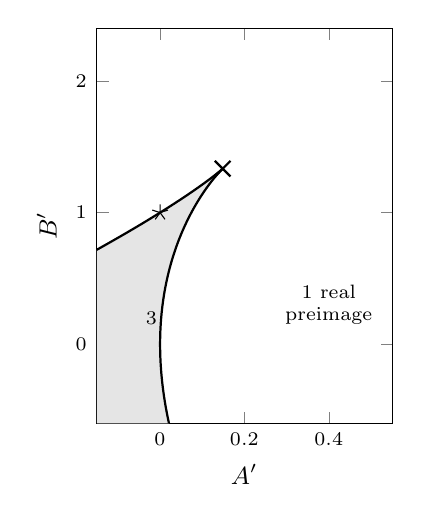
\begin{tikzpicture}\begin{axis}[width=0.44\linewidth, height=6.6cm, xlabel={$A'$}, ylabel={$B'$},
  xmin=-0.15, xmax=0.55, ymin=-0.6, ymax=2.4,
  tick label style={font=\scriptsize}, label style={font=\small}, clip=true]
\addplot[fill=black!10, draw=none] coordinates {(-1.01364,-0.60000) (-0.99012,-0.56791) (-0.96690,-0.53609) (-0.94398,-0.50454) (-0.92136,-0.47326) (-0.89904,-0.44225) (-0.87702,-0.41150) (-0.85529,-0.38102) (-0.83385,-0.35082) (-0.81271,-0.32088) (-0.79185,-0.29120) (-0.77128,-0.26180) (-0.75100,-0.23267) (-0.73099,-0.20380) (-0.71127,-0.17521) (-0.69183,-0.14688) (-0.67267,-0.11882) (-0.65379,-0.09102) (-0.63518,-0.06350) (-0.61684,-0.03625) (-0.59877,-0.00926) (-0.58097,0.01746) (-0.56344,0.04391) (-0.54618,0.07009) (-0.52918,0.09600) (-0.51244,0.12164) (-0.49596,0.14702) (-0.47974,0.17212) (-0.46377,0.19696) (-0.44806,0.22153) (-0.43261,0.24583) (-0.41740,0.26986) (-0.40245,0.29363) (-0.38774,0.31712) (-0.37328,0.34035) (-0.35906,0.36331) (-0.34508,0.38600) (-0.33134,0.40842) (-0.31785,0.43057) (-0.30459,0.45245) (-0.29156,0.47407) (-0.27877,0.49542) (-0.26621,0.51650) (-0.25388,0.53731) (-0.24177,0.55785) (-0.22989,0.57812) (-0.21824,0.59813) (-0.20681,0.61786) (-0.19560,0.63733) (-0.18461,0.65653) (-0.17383,0.67546) (-0.16328,0.69412) (-0.15293,0.71251) (-0.14280,0.73064) (-0.13287,0.74850) (-0.12316,0.76608) (-0.11365,0.78340) (-0.10434,0.80045) (-0.09524,0.81724) (-0.08634,0.83375) (-0.07763,0.84999) (-0.06913,0.86597) (-0.06082,0.88168) (-0.05270,0.89712) (-0.04478,0.91229) (-0.03704,0.92719) (-0.02950,0.94183) (-0.02214,0.95619) (-0.01496,0.97029) (-0.00797,0.98412) (-0.00116,0.99768) (0.00547,1.01097) (0.01192,1.02399) (0.01820,1.03675) (0.02431,1.04923) (0.03024,1.06145) (0.03600,1.07340) (0.04159,1.08508) (0.04702,1.09649) (0.05228,1.10764) (0.05738,1.11851) (0.06232,1.12912) (0.06709,1.13946) (0.07171,1.14953) (0.07618,1.15933) (0.08049,1.16886) (0.08464,1.17812) (0.08865,1.18712) (0.09251,1.19585) (0.09622,1.20430) (0.09978,1.21249) (0.10321,1.22041) (0.10649,1.22807) (0.10963,1.23545) (0.11263,1.24257) (0.11550,1.24941) (0.11823,1.25599) (0.12083,1.26230) (0.12330,1.26835) (0.12564,1.27412) (0.12785,1.27962) (0.12994,1.28486) (0.13190,1.28983) (0.13374,1.29453) (0.13546,1.29896) (0.13707,1.30312) (0.13855,1.30701) (0.13992,1.31064) (0.14118,1.31399) (0.14233,1.31708) (0.14337,1.31990) (0.14430,1.32245) (0.14513,1.32473) (0.14585,1.32675) (0.14647,1.32849) (0.14699,1.32997) (0.14741,1.33118) (0.14773,1.33212) (0.14796,1.33279) (0.14810,1.33319) (0.14815,1.33333) (0.14810,1.33319) (0.14797,1.33279) (0.14775,1.33212) (0.14745,1.33118) (0.14706,1.32997) (0.14660,1.32849) (0.14606,1.32675) (0.14544,1.32473) (0.14474,1.32245) (0.14397,1.31990) (0.14313,1.31708) (0.14222,1.31399) (0.14124,1.31064) (0.14020,1.30701) (0.13909,1.30312) (0.13792,1.29896) (0.13668,1.29453) (0.13539,1.28983) (0.13404,1.28486) (0.13264,1.27962) (0.13118,1.27412) (0.12967,1.26835) (0.12811,1.26230) (0.12651,1.25599) (0.12485,1.24941) (0.12316,1.24257) (0.12141,1.23545) (0.11963,1.22807) (0.11781,1.22041) (0.11595,1.21249) (0.11406,1.20430) (0.11213,1.19585) (0.11017,1.18712) (0.10818,1.17812) (0.10616,1.16886) (0.10412,1.15933) (0.10204,1.14953) (0.09995,1.13946) (0.09784,1.12912) (0.09570,1.11851) (0.09355,1.10764) (0.09138,1.09649) (0.08920,1.08508) (0.08701,1.07340) (0.08480,1.06145) (0.08259,1.04923) (0.08037,1.03675) (0.07815,1.02399) (0.07592,1.01097) (0.07369,0.99768) (0.07146,0.98412) (0.06923,0.97029) (0.06701,0.95619) (0.06479,0.94183) (0.06258,0.92719) (0.06038,0.91229) (0.05819,0.89712) (0.05601,0.88168) (0.05385,0.86597) (0.05170,0.84999) (0.04958,0.83375) (0.04747,0.81724) (0.04538,0.80045) (0.04332,0.78340) (0.04129,0.76608) (0.03928,0.74850) (0.03730,0.73064) (0.03535,0.71251) (0.03343,0.69412) (0.03155,0.67546) (0.02970,0.65653) (0.02789,0.63733) (0.02613,0.61786) (0.02440,0.59813) (0.02272,0.57812) (0.02108,0.55785) (0.01949,0.53731) (0.01795,0.51650) (0.01645,0.49542) (0.01501,0.47407) (0.01363,0.45245) (0.01230,0.43057) (0.01103,0.40842) (0.00982,0.38600) (0.00867,0.36331) (0.00758,0.34035) (0.00656,0.31712) (0.00560,0.29363) (0.00472,0.26986) (0.00390,0.24583) (0.00316,0.22153) (0.00249,0.19696) (0.00189,0.17212) (0.00138,0.14702) (0.00094,0.12164) (0.00058,0.09600) (0.00031,0.07009) (0.00012,0.04391) (0.00002,0.01746) (0.00001,-0.00926) (0.00008,-0.03625) (0.00025,-0.06350) (0.00051,-0.09102) (0.00087,-0.11882) (0.00132,-0.14688) (0.00188,-0.17521) (0.00253,-0.20380) (0.00329,-0.23267) (0.00415,-0.26180) (0.00512,-0.29120) (0.00620,-0.32088) (0.00738,-0.35082) (0.00868,-0.38102) (0.01009,-0.41150) (0.01162,-0.44225) (0.01326,-0.47326) (0.01503,-0.50454) (0.01691,-0.53609) (0.01892,-0.56791) (0.02105,-0.60000)} -- cycle;
\addplot[thick, black] coordinates {(0.14815,1.33333) (0.14810,1.33319) (0.14797,1.33279) (0.14775,1.33212) (0.14745,1.33118) (0.14706,1.32997) (0.14660,1.32849) (0.14606,1.32675) (0.14544,1.32473) (0.14474,1.32245) (0.14397,1.31990) (0.14313,1.31708) (0.14222,1.31399) (0.14124,1.31064) (0.14020,1.30701) (0.13909,1.30312) (0.13792,1.29896) (0.13668,1.29453) (0.13539,1.28983) (0.13404,1.28486) (0.13264,1.27962) (0.13118,1.27412) (0.12967,1.26835) (0.12811,1.26230) (0.12651,1.25599) (0.12485,1.24941) (0.12316,1.24257) (0.12141,1.23545) (0.11963,1.22807) (0.11781,1.22041) (0.11595,1.21249) (0.11406,1.20430) (0.11213,1.19585) (0.11017,1.18712) (0.10818,1.17812) (0.10616,1.16886) (0.10412,1.15933) (0.10204,1.14953) (0.09995,1.13946) (0.09784,1.12912) (0.09570,1.11851) (0.09355,1.10764) (0.09138,1.09649) (0.08920,1.08508) (0.08701,1.07340) (0.08480,1.06145) (0.08259,1.04923) (0.08037,1.03675) (0.07815,1.02399) (0.07592,1.01097) (0.07369,0.99768) (0.07146,0.98412) (0.06923,0.97029) (0.06701,0.95619) (0.06479,0.94183) (0.06258,0.92719) (0.06038,0.91229) (0.05819,0.89712) (0.05601,0.88168) (0.05385,0.86597) (0.05170,0.84999) (0.04958,0.83375) (0.04747,0.81724) (0.04538,0.80045) (0.04332,0.78340) (0.04129,0.76608) (0.03928,0.74850) (0.03730,0.73064) (0.03535,0.71251) (0.03343,0.69412) (0.03155,0.67546) (0.02970,0.65653) (0.02789,0.63733) (0.02613,0.61786) (0.02440,0.59813) (0.02272,0.57812) (0.02108,0.55785) (0.01949,0.53731) (0.01795,0.51650) (0.01645,0.49542) (0.01501,0.47407) (0.01363,0.45245) (0.01230,0.43057) (0.01103,0.40842) (0.00982,0.38600) (0.00867,0.36331) (0.00758,0.34035) (0.00656,0.31712) (0.00560,0.29363) (0.00472,0.26986) (0.00390,0.24583) (0.00316,0.22153) (0.00249,0.19696) (0.00189,0.17212) (0.00138,0.14702) (0.00094,0.12164) (0.00058,0.09600) (0.00031,0.07009) (0.00012,0.04391) (0.00002,0.01746) (0.00001,-0.00926) (0.00008,-0.03625) (0.00025,-0.06350) (0.00051,-0.09102) (0.00087,-0.11882) (0.00132,-0.14688) (0.00188,-0.17521) (0.00253,-0.20380) (0.00329,-0.23267) (0.00415,-0.26180) (0.00512,-0.29120) (0.00620,-0.32088) (0.00738,-0.35082) (0.00868,-0.38102) (0.01009,-0.41150) (0.01162,-0.44225) (0.01326,-0.47326) (0.01503,-0.50454) (0.01691,-0.53609) (0.01892,-0.56791) (0.02105,-0.60000)};
\addplot[thick, black] coordinates {(0.14815,1.33333) (0.14810,1.33319) (0.14796,1.33279) (0.14773,1.33212) (0.14741,1.33118) (0.14699,1.32997) (0.14647,1.32849) (0.14585,1.32675) (0.14513,1.32473) (0.14430,1.32245) (0.14337,1.31990) (0.14233,1.31708) (0.14118,1.31399) (0.13992,1.31064) (0.13855,1.30701) (0.13707,1.30312) (0.13546,1.29896) (0.13374,1.29453) (0.13190,1.28983) (0.12994,1.28486) (0.12785,1.27962) (0.12564,1.27412) (0.12330,1.26835) (0.12083,1.26230) (0.11823,1.25599) (0.11550,1.24941) (0.11263,1.24257) (0.10963,1.23545) (0.10649,1.22807) (0.10321,1.22041) (0.09978,1.21249) (0.09622,1.20430) (0.09251,1.19585) (0.08865,1.18712) (0.08464,1.17812) (0.08049,1.16886) (0.07618,1.15933) (0.07171,1.14953) (0.06709,1.13946) (0.06232,1.12912) (0.05738,1.11851) (0.05228,1.10764) (0.04702,1.09649) (0.04159,1.08508) (0.03600,1.07340) (0.03024,1.06145) (0.02431,1.04923) (0.01820,1.03675) (0.01192,1.02399) (0.00547,1.01097) (-0.00116,0.99768) (-0.00797,0.98412) (-0.01496,0.97029) (-0.02214,0.95619) (-0.02950,0.94183) (-0.03704,0.92719) (-0.04478,0.91229) (-0.05270,0.89712) (-0.06082,0.88168) (-0.06913,0.86597) (-0.07763,0.84999) (-0.08634,0.83375) (-0.09524,0.81724) (-0.10434,0.80045) (-0.11365,0.78340) (-0.12316,0.76608) (-0.13287,0.74850) (-0.14280,0.73064) (-0.15293,0.71251) (-0.16328,0.69412) (-0.17383,0.67546) (-0.18461,0.65653) (-0.19560,0.63733) (-0.20681,0.61786) (-0.21824,0.59813) (-0.22989,0.57812) (-0.24177,0.55785) (-0.25388,0.53731) (-0.26621,0.51650) (-0.27877,0.49542) (-0.29156,0.47407) (-0.30459,0.45245) (-0.31785,0.43057) (-0.33134,0.40842) (-0.34508,0.38600) (-0.35906,0.36331) (-0.37328,0.34035) (-0.38774,0.31712) (-0.40245,0.29363) (-0.41740,0.26986) (-0.43261,0.24583) (-0.44806,0.22153) (-0.46377,0.19696) (-0.47974,0.17212) (-0.49596,0.14702) (-0.51244,0.12164) (-0.52918,0.09600) (-0.54618,0.07009) (-0.56344,0.04391) (-0.58097,0.01746) (-0.59877,-0.00926) (-0.61684,-0.03625) (-0.63518,-0.06350) (-0.65379,-0.09102) (-0.67267,-0.11882) (-0.69183,-0.14688) (-0.71127,-0.17521) (-0.73099,-0.20380) (-0.75100,-0.23267) (-0.77128,-0.26180) (-0.79185,-0.29120) (-0.81271,-0.32088) (-0.83385,-0.35082) (-0.85529,-0.38102) (-0.87702,-0.41150) (-0.89904,-0.44225) (-0.92136,-0.47326) (-0.94398,-0.50454) (-0.96690,-0.53609) (-0.99012,-0.56791) (-1.01364,-0.60000)};
\addplot[only marks, mark=triangle*, mark size=3pt, mark options={fill=black}, draw=black] coordinates {(-16.00000,-16.00000)};
\addplot[only marks, mark=square*, mark size=3pt, mark options={fill=white}, draw=black] coordinates {(10.00000,0.00000) (0.00000,5.00000) (-3.00000,-2.00000) (2.00000,-0.66667) (-45.00000,21.00000)};
\addplot[only marks, mark=star, mark size=3pt, mark options={fill=black}, draw=black] coordinates {(0.00000,1.00000)};
\addplot[only marks, mark=x, mark size=4pt, thick, black] coordinates {(0.14815,1.33333)};
\node[font=\scriptsize, align=center] at (axis cs:0.4,0.3) {1 real\\preimage};
\node[font=\scriptsize, align=center] at (axis cs:-0.02,0.2) {3};
\end{axis}\end{tikzpicture}

\caption{The discriminant wall $\Sigma = 0$ of the announced map in the chart $C = 1$ with coordinates $A' = AC^2$ and $B' = BC$, which preserves the wall and the regions because $\Sigma(AC^2, BC, 1) = C^2\,\Sigma(A,B,C)$. Left: the whole range of the sampled targets; right: the neighborhood of the cusp at $(\numWallCuspA, \numWallCuspB)$. The shaded region ($D > 0$) has three real preimages; outside it there is one. Triangles are sampled targets with three real preimages, squares with one, the star is the escape target $(0,1,1)$, and the cross at the cusp is the point of $\Gamma$ in this chart, which the image omits. The curves are drawn from the exact polynomial of \eqref{eq:sigma}.}
\label{fig:wall}
\end{figure}

Figure~\ref{fig:fiber} shows the cubic behind the census, Figure~\ref{fig:wall} the wall that separates the regions, and Figure~\ref{fig:plane} the fibers over the plane $C = 0$. The cusp of the wall at $(\tfrac{4}{27}, \tfrac43)$ is the point of $\Gamma$ in the chart $C = 1$, where the three roots of $W$ coalesce.

\begin{figure}[t]\centering
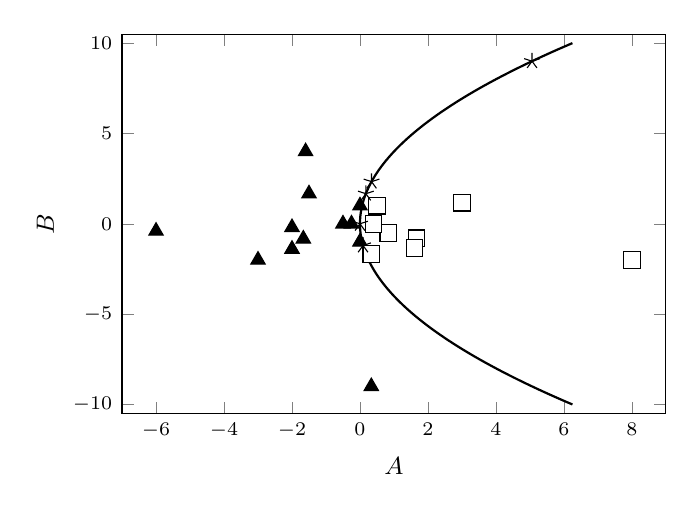
\begin{tikzpicture}
\begin{axis}[width=0.7\linewidth, height=6.4cm, xlabel={$A$}, ylabel={$B$}, xmin=-7, xmax=9, ymin=-10.5, ymax=10.5,
 tick label style={font=\scriptsize}, label style={font=\small}]
\addplot[thick, black] coordinates {(6.2500,-10.0000) (6.0434,-9.8333) (5.8403,-9.6667) (5.6406,-9.5000) (5.4444,-9.3333) (5.2517,-9.1667) (5.0625,-9.0000) (4.8767,-8.8333) (4.6944,-8.6667) (4.5156,-8.5000) (4.3403,-8.3333) (4.1684,-8.1667) (4.0000,-8.0000) (3.8351,-7.8333) (3.6736,-7.6667) (3.5156,-7.5000) (3.3611,-7.3333) (3.2101,-7.1667) (3.0625,-7.0000) (2.9184,-6.8333) (2.7778,-6.6667) (2.6406,-6.5000) (2.5069,-6.3333) (2.3767,-6.1667) (2.2500,-6.0000) (2.1267,-5.8333) (2.0069,-5.6667) (1.8906,-5.5000) (1.7778,-5.3333) (1.6684,-5.1667) (1.5625,-5.0000) (1.4601,-4.8333) (1.3611,-4.6667) (1.2656,-4.5000) (1.1736,-4.3333) (1.0851,-4.1667) (1.0000,-4.0000) (0.9184,-3.8333) (0.8403,-3.6667) (0.7656,-3.5000) (0.6944,-3.3333) (0.6267,-3.1667) (0.5625,-3.0000) (0.5017,-2.8333) (0.4444,-2.6667) (0.3906,-2.5000) (0.3403,-2.3333) (0.2934,-2.1667) (0.2500,-2.0000) (0.2101,-1.8333) (0.1736,-1.6667) (0.1406,-1.5000) (0.1111,-1.3333) (0.0851,-1.1667) (0.0625,-1.0000) (0.0434,-0.8333) (0.0278,-0.6667) (0.0156,-0.5000) (0.0069,-0.3333) (0.0017,-0.1667) (0.0000,0.0000) (0.0017,0.1667) (0.0069,0.3333) (0.0156,0.5000) (0.0278,0.6667) (0.0434,0.8333) (0.0625,1.0000) (0.0851,1.1667) (0.1111,1.3333) (0.1406,1.5000) (0.1736,1.6667) (0.2101,1.8333) (0.2500,2.0000) (0.2934,2.1667) (0.3403,2.3333) (0.3906,2.5000) (0.4444,2.6667) (0.5017,2.8333) (0.5625,3.0000) (0.6267,3.1667) (0.6944,3.3333) (0.7656,3.5000) (0.8403,3.6667) (0.9184,3.8333) (1.0000,4.0000) (1.0851,4.1667) (1.1736,4.3333) (1.2656,4.5000) (1.3611,4.6667) (1.4601,4.8333) (1.5625,5.0000) (1.6684,5.1667) (1.7778,5.3333) (1.8906,5.5000) (2.0069,5.6667) (2.1267,5.8333) (2.2500,6.0000) (2.3767,6.1667) (2.5069,6.3333) (2.6406,6.5000) (2.7778,6.6667) (2.9184,6.8333) (3.0625,7.0000) (3.2101,7.1667) (3.3611,7.3333) (3.5156,7.5000) (3.6736,7.6667) (3.8351,7.8333) (4.0000,8.0000) (4.1684,8.1667) (4.3403,8.3333) (4.5156,8.5000) (4.6944,8.6667) (4.8767,8.8333) (5.0625,9.0000) (5.2517,9.1667) (5.4444,9.3333) (5.6406,9.5000) (5.8403,9.6667) (6.0434,9.8333) (6.2500,10.0000)};
\addplot[only marks, mark=triangle*, mark size=3pt, mark options={fill=black}, draw=black] coordinates {(0.0000,1.0000) (-0.2500,0.0000) (-6.0000,-0.4000) (-2.0000,-1.4000) (-1.6000,4.0000) (-3.0000,-2.0000) (-1.5000,1.6667) (-2.0000,-0.2000) (0.3333,-9.0000) (-0.5000,0.0000) (0.0000,-1.0000) (-1.6667,-0.8333)};
\addplot[only marks, mark=square*, mark size=3pt, mark options={fill=white}, draw=black] coordinates {(0.8333,-0.5000) (3.0000,1.1667) (0.3333,-1.6667) (1.6667,-0.8000) (0.4000,0.0000) (0.5000,1.0000) (8.0000,-2.0000) (1.6000,-1.3333)};
\addplot[only marks, mark=star, mark size=3pt, mark options={fill=black}, draw=black] coordinates {(0.3403,2.3333) (0.0900,-1.2000) (0.1736,1.6667) (0.0000,0.0000) (5.0625,9.0000)};

\end{axis}
\end{tikzpicture}
\caption{The \numPlaneTargets{} sampled targets $(A,B,0)$ of computation EXP-145 and the parabola $B^2 = 16A$ (curve). Triangles: $B^2 > 16A$, three real preimages; squares: $B^2 < 16A$, one real and two non-real preimages; stars: $B^2 = 16A$, the single flat-sheet point. Each marker is the fiber size reported in the stored output, three off the parabola and one on it.}
\label{fig:plane}
\end{figure}

\section{The two-dimensional frontier}\label{sec:planar}

\subsection{The obstruction to the mechanism (EXP-005)}\label{sec:obstruction}

\begin{theorem}[{\MV} with generic symbolic $f, g$; {\DD} for all weights]\label{thm:2d}
Let $\Gm$ act on $\C^2$ with weights $(1, -a)$, $a \ge 1$, and let $F = (x^{b_1} f(v),\,
x^{b_2} g(v))$, $v = x^a y$, be an equivariant polynomial map. Then
\begin{equation}\label{eq:det2d}
\detJ = x^{\,b_1 + b_2 + a - 1}\left(b_1 f g' - b_2 f' g\right),
\end{equation}
so the Keller condition forces $b_1 + b_2 = 1 - a$ and the single univariate identity
$b_1 f g' - b_2 f' g = \mathrm{const} \ne 0$.
\end{theorem}
\begin{proof}
$P_x = x^{b_1-1}(b_1 f + a v f')$, $P_y = x^{b_1+a}f'$, $Q_x = x^{b_2-1}(b_2 g + a v g')$, $Q_y = x^{b_2+a}g'$. Then $P_xQ_y - P_yQ_x = x^{b_1+b_2+a-1}\bigl[b_1fg' + a v f'g' - b_2f'g - a v f'g'\bigr]$. The bracket is a polynomial in $v$ alone and the prefactor is a pure power of $x$, so a nonzero constant determinant forces the exponent to vanish and the bracket to be constant.
\end{proof}

The identity was also certified for $a \in \{1,2,3\}$ and several windows of $(b_1,b_2)$ with symbolic $f, g$ \MV. The three-dimensional family has no counterpart:

\begin{proposition}[One-invariant collapse, {\DD}]\label{prop:collapse}
If the reduced data $(V', T')$ of a weighted skew product depend on a single variable, then
$dV' \wedge dT' = 0$, hence $J_2 \equiv 0$ and $\detJ \equiv 0$: no Keller map arises. Since a
nontrivial $\Gm$-action on $\C^2$ has one independent weight-zero invariant (against two in
$\C^3$), the potential-form mechanism of Theorem~\ref{thm:family} is structurally unavailable in
dimension $2$.
\end{proposition}

Additionally \MV: no coordinate slice of \eqref{eq:F} (each variable frozen at three rational test values, any output pair) is a planar Keller map, so $F$ does not hide a planar Keller map in a slice; slices by non-coordinate planes are not excluded.

\subsection{Equivariant rigidity}\label{sec:rigidity}

\begin{theorem}[Planar equivariant rigidity, {\DD}; every mechanical step {\MV} on sweeps]\label{thm:rigidity}
Let $\Gm$ act on $\C^2$ with weights $(w_1, -w_2)$, $w_1 \ge 1$, $w_2 \ge 0$, and let $F = (P,Q)$ be a polynomial Keller map whose components are weight vectors.
\begin{enumerate}
\item If $w_2 \ge 1$, then $F$ is linear: $(f_0 x,\, g_0 y)$ or $(f_0 y,\, g_0 x)$ with $f_0 g_0 \neq 0$.
\item If $w_2 = 0$, then $F$ is affine: $(f_0 x,\, g_0 y + c)$ or $(f_0 y + c,\, g_0 x)$ with $f_0 g_0 \ne 0$, linear exactly when $c = 0$.
\end{enumerate}
\end{theorem}

\begin{proof}
\emph{Weights $(w_1, 0)$.} A monomial $x^iy^j$ has weight $iw_1$, so $P = x^{i}f(y)$ and $Q = x^{i'}g(y)$ for integers $i, i' \ge 0$, and $\detJ = x^{i+i'-1}(i f g' - i' f' g)$. The bracket is a polynomial in $y$. If $i + i' \ge 2$ the determinant vanishes on $x = 0$; if $i = i' = 0$ it is zero; so $i + i' = 1$. For $(i,i') = (1,0)$ the determinant is $f g'$, a nonzero constant exactly when $f = f_0 \neq 0$ is constant and $g = g_0y + c$ with $g_0 \neq 0$; for $(0,1)$ it is $-f'g$ and the roles are exchanged. The map $(x, y + 1)$ shows that the translation occurs.

\emph{Weights $(w_1, -w_2)$ with $w_2 \ge 1$.} Dividing both weights by their greatest common divisor changes neither the weight spaces nor the invariants, so assume $\gcd(w_1,w_2) = 1$. The monomials $x^iy^j$ of one weight satisfy $w_1 i - w_2 j = \mathrm{const}$, so they differ by multiples of $(w_2, w_1)$, and
$P = x^{i_1}y^{j_1} f(v)$, $Q = x^{i_2}y^{j_2} g(v)$ with $v = x^{w_2}y^{w_1}$ and $f, g \in \C[v]$ nonzero. A direct computation of the four partial derivatives gives
\begin{equation}\label{eq:det2dgen}
\detJ = x^{i_1 + i_2 - 1}\, y^{j_1 + j_2 - 1}\, B(v), \qquad
B = (i_1 j_2 - i_2 j_1)\, f g + v\,(\beta_1 f g' - \beta_2 f' g), \quad \beta_r = w_1 i_r - w_2 j_r .
\end{equation}
Write $a = i_1 + i_2 - 1 \ge -1$, $b = j_1 + j_2 - 1 \ge -1$ and $B = \sum_n B_nv^n$. Then $\detJ = \sum_n B_n\,x^{a + nw_2}y^{b + nw_1}$ with pairwise distinct monomials, so a nonzero constant means that a single $B_n \neq 0$ and $a + nw_2 = b + nw_1 = 0$. If $n \ge 1$ then $a = -nw_2 \le -1$, so $a = -1$, $n = w_2 = 1$ and likewise $b = -1$, $w_1 = 1$; then $i_1 = i_2 = j_1 = j_2 = 0$, $\beta_1 = \beta_2 = 0$ and $B \equiv 0$, a contradiction. Hence $n = 0$, $a = b = 0$ and $B$ is a nonzero constant: $i_1 + i_2 = j_1 + j_2 = 1$. The four resulting shapes are $(xf, yg)$, $(yf, xg)$, $(xyf, g)$ and $(f, xyg)$. For the last two $i_1j_2 - i_2j_1 = 0$, so $B$ is divisible by $v$ and cannot be a nonzero constant. For $(xf, yg)$, $B = fg + v(w_1fg' + w_2f'g)$; for $(yf, xg)$, $B = -fg - v(w_2fg' + w_1f'g)$. Let $d_f$ and $d_g$ be the degrees of $f$ and $g$ and $N = d_f + d_g$. In the first case the coefficient of $v^N$ in $B$ is $(1 + w_1d_g + w_2d_f)\,f_{d_f}\,g_{d_g}$, and in the second it is $-(1 + w_2d_g + w_1d_f)\,f_{d_f}\,g_{d_g}$. The factor in parentheses is a positive integer and $f_{d_f}g_{d_g} \neq 0$, so the coefficient is nonzero; as $B$ is constant, $N = 0$. Thus $f$ and $g$ are constants and $F$ is $(f_0 x, g_0 y)$ or $(f_0 y, g_0 x)$.
\end{proof}

The top-coefficient argument forces $d_f + d_g = 0$ directly, with no descent. The mechanical steps are certified. The determinant factorization \eqref{eq:det2dgen} holds in \numRigCases{} cases (the \numWeightPairs{} weight pairs \weightPairs{}, including the semi-trivial pair $(1,0)$, times all exponent vectors in $[0,2]^4$, with generic symbolic cubic $f, g$) \MV. The mixed shapes have no Keller solution at degrees up to $4$ for the whole weight sweep, the surviving shapes have only constant solutions for all exact bidegrees up to \numSweepDeg{}, as exact emptiness of constrained polynomial systems over $\Q$ with the leading coefficients and the constant imposed nonzero, and the positivity of the factor $1 + w_1d_g + w_2d_f$ is checked for all degrees up to \numKillDeg{} \MV.

The independent enumeration of Algorithm~\ref{alg:enum} (\numEnumInst{} polynomial Keller instances over the bounded window, from \numBranches{} branches, with \numBadResidual{} parameter instantiations discarded by the residual test, all \numEnumFibers{} exactly computed in-image fibers single-point, and exactly \numShapes{} instance shapes, every one linear \MV) is the experimental companion of Theorem~\ref{thm:rigidity}; Figure~\ref{fig:window} shows in which cells of the window the instances occur.

\begin{figure}[t]\centering
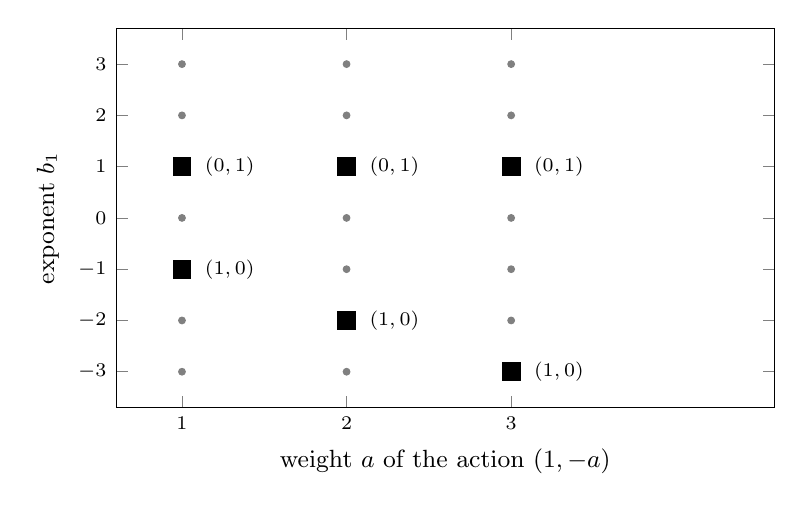
\begin{tikzpicture}
\begin{axis}[width=0.82\linewidth, height=6.4cm, xlabel={weight $a$ of the action $(1,-a)$}, ylabel={exponent $b_1$}, xmin=0.6, xmax=4.6, ymin=-3.7, ymax=3.7,
 xtick={1,2,3}, ytick={-3,-2,-1,0,1,2,3}, tick label style={font=\scriptsize}, label style={font=\small}]
\addplot[only marks, mark=*, mark size=1.2pt, gray] coordinates {(1,-3) (1,-2) (1,-1) (1,0) (1,1) (1,2) (1,3) (2,-3) (2,-2) (2,-1) (2,0) (2,1) (2,2) (2,3) (3,-3) (3,-2) (3,-1) (3,0) (3,1) (3,2) (3,3)};
\addplot[only marks, mark=square*, mark size=3.2pt, black] coordinates {(1,-1) (1,1) (2,-2) (2,1) (3,-3) (3,1)};
\node[font=\scriptsize, anchor=west] at (axis cs:1.08,-1.0) {$(1,0)$};
\node[font=\scriptsize, anchor=west] at (axis cs:1.08,1.0) {$(0,1)$};
\node[font=\scriptsize, anchor=west] at (axis cs:2.08,-2.0) {$(1,0)$};
\node[font=\scriptsize, anchor=west] at (axis cs:2.08,1.0) {$(0,1)$};
\node[font=\scriptsize, anchor=west] at (axis cs:3.08,-3.0) {$(1,0)$};
\node[font=\scriptsize, anchor=west] at (axis cs:3.08,1.0) {$(0,1)$};

\end{axis}
\end{tikzpicture}
\caption{Cells $(a, b_1)$ of the enumeration window (small dots) and the cells in which polynomial equivariant Keller maps of $\C^2$ exist (squares), read from the stored output of EXP-006, each labeled with the degrees $(\deg f, \deg g)$ of the instance shape; every instance is linear, so the squares are the diagonal and swap shapes of Theorem~\ref{thm:rigidity}.}
\label{fig:window}
\end{figure}

Consequence: a two-variable counterexample, if one exists, must be non-equivariant for every weight choice with $w_2 \ge 0$; the symmetry class behind the three-dimensional family is closed in dimension two.

\subsection{Scope and independent classification}\label{sec:scope}

The word ``linear'' in Theorem~\ref{thm:rigidity} is restricted to opposite-sign weights; with one zero weight the maps are affine, in agreement with the classification of \cite{Shaska2026}. Same-sign actions admit nonlinear triangular equivariant automorphisms. Shaska, in work submitted on 2026-07-22, proves the full classification: triangular automorphisms for same-sign weights, affine automorphisms when one weight is zero, and linear automorphisms for opposite-sign weights \VV{}; the proof there is independent of the sweeps above and uses the invariant $m = x^qy^p$ and a degree identity that forces $\deg A + \deg B = 0$. Every equivariant planar Keller map is therefore an automorphism in every signature. We make no priority or novelty claim for the classification. The contribution here is the determinant factorization \eqref{eq:det2dgen}, the exact computations on the hyperbolic scope relevant to the three-dimensional mechanism, and the remark that the three-dimensional family has no planar analogue.

The remaining routes to a hypothetical two-dimensional counterexample are no symmetry at all; non-reductive ($\mathbb{G}_a$) structures, which face the same one-invariant collapse in naive form; and gradings at infinity in the Newton-polygon sense. A proof of $JC(2)$ in these terms is a properness statement: the reconstruction \eqref{eq:reconstruct} shows how asymptotic values are produced in dimension three, through denominators $BC = k^2p(w)$, and whether one-invariant geometry in the plane leaves room for such an escape is the question that the three-dimensional mechanism leaves open for $JC(2)$.

\section{Ablation of the mechanism}\label{sec:ablation}

\subsection{Components of the construction}

Four ingredients make the family work, and each one has been removed in an exact computation.
\begin{enumerate}
\item \emph{The second weight-zero invariant.} With a single invariant the reduced pair depends on one variable and $J_2 \equiv 0$ (Proposition~\ref{prop:collapse}): no Keller map arises. This is the planar case.
\item \emph{The potential form.} Replacing it by the first constructor (Proposition~\ref{prop:first}) leaves one rigid shape at degree two and no instance at degrees three and four.
\item \emph{The admissibility conditions.} They are necessary and sufficient for the polynomiality of the lifted map (Step~2 of the proof of Theorem~\ref{thm:family}); a seed that violates one gives a rational map that is not a polynomial map.
\item \emph{The scale and the section tail.} They do not enter the determinant $-k\,p(1)^2$ beyond the factor $k$, and they change only the degrees: $k = 7$ leaves them unchanged at $d = 2$, a tail raises them (Theorem~\ref{thm:degrees}).
\end{enumerate}
The result is that the weight system and the potential form carry the mechanism, while the seed degree, the scale and the tail are free axes of a single family.

\subsection{Other weight systems (EXP-012)}

\begin{table}[t]\centering\small
\begin{tabular}{c>{\raggedright\arraybackslash}p{0.17\textwidth}>{\raggedright\arraybackslash}p{0.27\textwidth}>{\raggedright\arraybackslash}p{0.36\textwidth}}
\toprule
$m$ & Output weights $o$ & Class & Outcome \\
\midrule
1 & $(-1,-1,1)$ & reduced pair is a planar Keller map & 93 instances, every in-image fiber has at most one point \\
2 & $(-2,-1,1)$ & the mechanism of Section~\ref{sec:family} & the seed family of Table~\ref{tab:instances} \\
3 & $(-2,-2,1)$ & lattice-level scan & empty class (valuation argument) \\
3 & $(-3,-1,1)$ & lattice-level scan & 60 instances, every in-image fiber has at most one point \\
4 & $(-3,-2,1)$ & potential form $V'=k^2p(w)+\mu s^2$ & empty system (5 conditions, Gr\"obner basis $[1]$) \\
\bottomrule
\end{tabular}

\caption{Weight systems $(1,-1,-m)$ scanned for counterexample families, read from the stored outputs of EXP-012: the weight $m$, the output weights $o$, the class tested and the outcome. Only $m = 2$ yields a family that collides.}
\label{tab:landscape}
\end{table}

For source weights $(1, -1, -m)$ and components $F_i = x^{o_i} f_i(v,t)$, with $\sigma = o_1 + o_2 + o_3$, the determinant lemma and the pairing reductions
\begin{equation}\label{eq:landscape}
\detJ = x^{\sigma + m}\,D, \qquad J_2 = \pm\, c_1^{\,r_a + r_b - 1} D
\end{equation}
hold generically in all \numLemmaCases{} tested $(m, o)$ cases and for the four natural pairings \MV, so the reduced Jacobian vanishes to order $m - 1$ along the section. The survey outcome is Table~\ref{tab:landscape}. At $m = 1$ the reduced pair is itself a planar Keller map, so that class is a \emph{bridge} to $JC(2)$ (\numBridgeInst{} scanned instances over \numPatterns{} sparse patterns, all injective; a collision there would refute $JC(2)$). At $m = 3$ the class $o = (-2,-2,1)$ is \emph{empty}, by a one-line valuation argument that the lattice forbids $v$-linear monomials in both negative components, so $D(0,0) = 0$, machine-certified on a generic ansatz, and $o = (-3,-1,1)$ is rigid in scans (\numRigidInst{} instances). At $m = 4$ the potential-form family does \emph{not} exist: with seed degree up to \numSeedDegMax{} and gauge $Q_0 = 1$ the \numAdmissCond{} admissibility conditions have Gr\"obner basis $[1]$ under $\mu \neq 0$ \MV. A parity law that would give families at every even $m$ therefore fails: $m = 4$ admits no such family. Within the scanned weighted landscape the announced counterexample's weight system is the unique collision-capable mechanism. The scope is sparse bounded scans, quantified in the computation; wider weight systems and higher-degree seeds are not covered.

\section{Validation}\label{sec:validation}

Each theorem is checked by at least one route that does not reuse the step that produced it. Table~\ref{tab:validation} lists the routes and their numbers; every number is from a stored output.

\begin{table}[t]\centering\footnotesize
\begin{tabular}{>{\raggedright\arraybackslash}p{0.2\textwidth}>{\raggedright\arraybackslash}p{0.4\textwidth}>{\raggedright\arraybackslash}p{0.3\textwidth}}
\toprule
Result & Independent route & Numbers \\
\midrule
Theorem~\ref{thm:valid} & determinant by cofactor path and full expansion; fiber by Gr\"obner basis, independent of pointwise substitution; structural re-derivation (Theorem~\ref{thm:structure}); hand substitution \eqref{eq:hand} & $\det = \numDetF$; fiber of 3 points \\
Theorem~\ref{thm:structure} and Lemma~\ref{lem:skew} & determinant by $3\times 3$ expansion versus the reduced identity; fiber by Gr\"obner versus the cubic; chain-rule proof & $J_2 = 2c_1^2$; generic symbolic coefficients \\
Theorem~\ref{thm:family}, Theorem~\ref{thm:instances} & determinant computed in $(x,y,z)$ and from $J_2 = m^2c_1^2/k$; collisions by exact substitution into the full components, independent of the reconstruction; proof of Section~\ref{sec:constructor} & 5 instances; determinants $-2,-3,-350,-20,-2$ \\
Theorem~\ref{thm:degrees} & degrees by total degree of the expanded components; $k = 7$ and two tails & 4 seeds; 2 tails \\
Remark~\ref{rem:charp} & two primes; exact images in characteristic $0$, reduction with modular inverses, distinctness in $\mathbb{F}_\ell^3$ & $\ell = 13, 101$; degree $12$ \\
Theorems~\ref{thm:asymptotic}, \ref{thm:cplane} & polynomial identity, then fibers on and off the surface by Gr\"obner basis; fiber over $C = 0$ at the announced target and at $(0,1,0)$; symbolic parametrization and \numPlaneTargets{} plane targets with radicality by a squarefree eliminant (EXP-145) & $D(-16,-16,1) = \numDcollision$; 3 and 1 point fibers \\
Theorem~\ref{thm:realcensus} & Sturm route versus Gr\"obner route; grid of \numGrid{} targets; triple-root argument for $\Gamma$; unit Gr\"obner ideal over $\Gamma$ with a control; quotient dimension against simple-root count (EXP-145) & 6 targets, 2 regions; \numImgTargets{} targets \\
Theorem~\ref{thm:2d}, \ref{thm:rigidity} & symbolic identity with free $f,g$; enumeration of \numEnumInst{} instances against sweeps; the classification of \cite{Shaska2026}; the proof of Section~\ref{sec:rigidity} & \numRigCases{} cases, \numWeightPairs{} weight pairs; \numEnumFibers{} fibers \\
Table~\ref{tab:landscape} & Gr\"obner and valuation certificates for the empty classes; scans with in-image targets & \numBridgeInst{}, \numRigidInst{} instances; 5 conditions \\
\bottomrule
\end{tabular}
\caption{Validation of each result: the route that does not reuse the step that produced it, and the numbers read from the stored outputs. Rows are ordered as the results appear in the paper.}
\label{tab:validation}
\end{table}

Two observations bound the evidence. First, the identities certified with generic symbolic coefficients (the determinant lemma, the planar determinant factorization, the one-variable fiber identity) cover whole families, while the instance certificates (Table~\ref{tab:collisions}) cover specific maps and the proofs of Theorems~\ref{thm:family}, \ref{thm:cplane} and~\ref{thm:realcensus} cover the general case by argument. Second, the only software is sympy, so a defect in one library would affect every route that uses it; the exact-substitution checks of computation EXP-145, which do not depend on the Gr\"obner routine, the hand-checkable substitutions \eqref{eq:hand}, the closed forms \eqref{eq:closed} at $t = 0$ and the fibers over $C = 0$ reduce that dependence at the points where it matters most. The mixed-route design is the same throughout: each exact statement is established by a computation of one kind and checked by a computation of another kind, or by a proof.

The negative controls and the failed predictions are part of the validation. The first constructor fails for seeds of degree three and four, and the failure is an exact emptiness statement (Proposition~\ref{prop:first}). The first planar enumeration returned no instance, which proved nothing, and the valuation-aware enumeration of Algorithm~\ref{alg:enum} replaced it, with every discard counted. The parity law for weight systems predicted a family at $m = 4$ and was refuted by a Gr\"obner certificate, so the landscape of Table~\ref{tab:landscape} was shaped by a prediction that failed. The determinant lemma and the pairing reductions were checked in all \numLemmaCases{} cases before any scan relied on them.

Finally, the numbers quoted in the text are not typed by hand. The script \texttt{gen\_tables.py} reads each stored output, writes the numbers, the tables and the data of the figures, and fails when an expected line is absent from an output, so a change in a stored output changes the paper at the next build and cannot go unnoticed. The proofs of Sections~\ref{sec:constructor}, \ref{sec:asymptotic}, \ref{sec:real} and~\ref{sec:rigidity} are checked by hand against the same outputs: the closed forms \eqref{eq:closed} reproduce the stored polynomials of $F$ on $t = 0$, the formulas \eqref{eq:cplane} reproduce the three announced points, and the determinant factorization \eqref{eq:det2dgen} is the one certified in \numRigCases{} cases.

\section{Discussion and open problems}\label{sec:discussion}

\textbf{Why the conjecture is false.} In the equivariant class, being Keller is a two-variable potential identity, satisfiable for free at any fiber degree $\ge 3$; nothing in the determinant sees properness. \textbf{What is essential.} Two independent weight-zero invariants, the potential form and the valuation conditions at the origin (Section~\ref{sec:ablation}).

\textbf{Consequences for related conjectures.} The cascade paper \cite{SLcascade} tabulates, for each neighbouring conjecture, the implication with its dimension index, the evidence mark and an explicit witness; it is cited here by content. Three facts from the current table bear on this paper. (a) The Mathieu conjecture is false for $SU(N)$ for every $N \ge 15$: at fixed $N$ Mathieu's argument, as rendered in Zwart's review \cite{Zwart2025}~\VV{}, makes every Keller map $x - h$ of $\C^N$ with $h$ homogeneous invertible under the conjecture for $SU(N)$, and de Bondt's homogenization of the counterexample \cite{deBondt2026} gives such a non-invertible map on $\C^{15}$, of degree $7$, verified exactly in EXP-138 \MV; Mathieu's 1997 paper itself was not located \cite{Mathieu1997}~\UU{}. An explicit counterexample for $SU(2)$ is due to Long \cite{LongSU2}~\VV{}, with the identities checked exactly for the first twelve powers. For $3 \le N \le 14$ the question is open, since $F$ is not affinely of the form $x - h$; the abelian case is due to Duistermaat and van der Kallen \cite{DvdK1998}. (b) The Poisson conjecture is false for every index $n \ge 2$: Long gives explicit polynomials with Poisson brackets $\{D,R\} = \{S,T\} = 1$ and all other brackets zero that define a Poisson endomorphism of the canonical algebra in four variables that is not an automorphism, built from the announced map \cite{LongPoisson}~\VV{}; the index $1$ remains open, and because the implication $PC(n) \Rightarrow DC(n)$ runs from a false premise it gives no information on the Dixmier conjecture of rank $2$ \cite{AvdE2007}. (c) The smallest dimensions known for witnesses are those of de Bondt \cite{deBondt2026}~\VV{}: counterexamples to the homogeneous Jacobian conjecture in dimension $15$, to Zhao's vanishing conjecture in dimension $28$ and to its homogeneous form in dimension $30$, over the integers (the homogeneous Jacobian conjecture in dimension $15$) and over the Gaussian integers (dimensions $28$ and $30$); they supersede in dimension the $48$-variable symmetric witness of \cite{SLcascade}, which remains the independently verified one. The Gaussian moments conjecture is false in every dimension $n \ge 3$ \cite{DEZ2017, LongGMC} (a proof for $n = 2$ is claimed \cite{Wilson2026}~\UU{}); the full Dixmier conjecture is false ($\mathrm{Dixmier}(n)$ implies $JC(n)$, and the converse $JC(2n) \Rightarrow \mathrm{Dixmier}(n)$ \cite{BKK2007, Tsuchimoto2005} gives only stable equivalence, with ranks $1$ and $2$ open and a proof for rank $1$ claimed \cite{Zheglov2024}~\UU{}); Zhao's vanishing conjecture is false, being equivalent to $JC$; and the Image conjecture is false in some dimension, since it implies the vanishing conjecture \cite{vdE2010}.

\textbf{Open problems.} In the plane, the companion paper \cite{SLplanar} treats the transport closure of the fifth exclusion, the $B = 16$ normal form and the $(72,108)$ system. In dimension three, global minimality remains open: it is not known to the author whether a Keller counterexample of total degree $3$ to $6$ exists~\UU{}, and within the family the degree law and minimality are Conjecture~\ref{conj:degrees}. The image of $F$ omits the curve $\Gamma$, which has the maximal dimension allowed: for a dominant quasi-finite polynomial map of $\C^3$ the complement of the image has dimension at most $1$, because a dense open part of an irreducible surface $\{h = 0\}$ in the complement would give a hypersurface $F^{-1}\{h = 0\}$ (as $h \circ F$ is nonconstant) whose image is dense in $\{h = 0\}$, a contradiction.

\section{Limitations}\label{sec:limitations}

The limits of the evidence are the following.
\begin{enumerate}
\item The degree law and the minimality of the announced map rest on four seeds, one scale and two tails; the general statement is Conjecture~\ref{conj:degrees}.
\item The structure of the fibers over $C = 0$ (Theorem~\ref{thm:cplane}), the asymptotic variety as $\{\Sigma = 0\}$ and the image $\C^3 \setminus \Gamma$ (Theorem~\ref{thm:realcensus}) are derived by proof. Computation EXP-145 certifies the symbolic identities, the emptiness over $\Gamma$ exactly and \numImgTargets{} plus \numPlaneTargets{} sampled targets; it does not enumerate every target, so the statement that every target off $\Gamma$ has a preimage, and the asymptotic variety as a whole, rest on the proofs.
\item The weight-system survey is a sparse bounded scan; the uniqueness of the mechanism is a statement about the scanned landscape, with seed degree at most \numSeedDegMax{} for $m = 4$, specific output weights and specific pairings. A non-potential map at $m = 4$ is not excluded.
\item The planar results concern $\Gm$-equivariant maps only; non-equivariant planar Keller maps are untouched. The enumeration window is $a \le 3$, $|b_1| \le 3$, degrees at most $3$, and the sweeps cover \numWeightPairs{} weight pairs and bidegrees up to \numSweepDeg{}; the arbitrary-weight statement rests on the proof of Section~\ref{sec:rigidity}.
\item The determinant value $-k\,p(1)^2$ shows that every negative rational occurs; it gives no information on the size of the coefficients needed for a counterexample of small degree, and the degree vectors of Table~\ref{tab:instances} grow with the seed degree.
\item Fibers computed as the rational solutions of a Gr\"obner system omit irrational and complex points; the fiber over a generic rational target $(A,B,0)$ shows that this matters, and the statements about $C = 0$ above use the full solution set.
\item Mathieu's 1997 paper was not located, so the Mathieu implication is checked in Zwart's review only; the proofs of Wilson and Zheglov are not verified, and Long's Poisson counterexample is read in the primary text but not re-verified here.
\item The only software is sympy; versions are recorded for EXP-001 and EXP-145; the only archived wall time is that of EXP-145. Non-coordinate planar slices of $F$ are not excluded from being planar Keller maps.
\item The real census samples six targets and a grid; it certifies that the two routes agree there and that both census values occur, while the structure of the regions and of the image is established by the argument of Theorem~\ref{thm:realcensus} and not by sampling.
\item The figures plot exact polynomials with floating-point coordinates for display; they carry no result that the text does not derive.
\end{enumerate}
These limits do not affect the validation of the announced map (Theorem~\ref{thm:valid}), the proof of the constructor (Theorem~\ref{thm:family}) or the classification of Section~\ref{sec:rigidity}, which are exact; they bound the claims about the degree law, the landscape of weight systems and the literature.

\section{Reproducibility and data availability}\label{sec:repro}

{\sloppy Every result labeled \MV{} is an exact sympy computation, over $\Q$ or, for the characteristic-$p$ statements (EXP-009), over $\mathbb{F}_\ell$, whose script and output are archived in the repository \url{https://github.com/fsantibanezleal/CAOS_RESEARCH}. An identifier EXP-$nnn$ denotes one archived computation in the experiment folders of the problem, \nolinkurl{problems/algebraic-geometry/jacobian-conjecture/experiments/}; each states its question, method and result, with the script and output of any computation. The results of this paper rest on EXP-001 through EXP-012, on EXP-145 (the image and the fibers over $C = 0$) and, for the discussion, on EXP-016 (the cited implications checked against their primary sources, except Mathieu's 1997 paper, which was not located), EXP-041 (the $48$-variable witness), EXP-136 (the dimension indices) and EXP-138 (the dimension-$15$ homogeneous witness). The tables, the numbers quoted from outputs and the data of the figures are regenerated from the stored outputs by the script \texttt{gen\_tables.py} in the manuscript folder (\texttt{python gen\_tables.py}, with \texttt{--check} to compare against the committed files), and the source builds with three runs of \texttt{pdflatex}.\par}

\section{Conclusions}\label{sec:conclusions}

The announced map has determinant $-2$ and a fiber of exactly three points over the announced target, and that fiber is the generic fiber over the plane $C = 0$. It is a weighted skew product whose Keller property is a two-variable identity and whose fibers are governed by a cubic. The potential form turns this into a proved constructor: every admissible seed, scale and section gives a Keller map of determinant $-k\,p(1)^2$ with an explicit reconstruction of the preimages, and the fiber degrees $3$ to $6$ occur with rational collisions. The degree law holds on four seeds and is conjectured beyond them. The asymptotic variety is the discriminant surface alone, the image omits the explicit curve $\Gamma$, and the real fibers have one or three points with the cusp of the wall at the point of $\Gamma$ in each normalized chart. In dimension two, equivariant Keller maps are linear or affine, so a planar counterexample must be non-equivariant, and the three-dimensional mechanism is unique among the weight systems scanned. The open questions are the proof of the degree law for all seeds, the existence of a counterexample of total degree $3$ to $6$ in dimension three, and $JC(2)$.

\begin{thebibliography}{99}
\raggedright
\bibitem{Alpoge2026} L. Alp\"oge, announcement of the counterexample, X (@\_\_alpoge\_\_),
2026-07-20; question posed by Akhil, map produced with Claude Fable 5. Independent press % voice-ok: external attribution, as the announcement states it
coverage: M. Sparkes, \emph{New Scientist}, 2026-07-20.
\bibitem{Wang1980} S. S.-S. Wang, A Jacobian criterion for separability, \emph{J. Algebra} \textbf{65} (1980), 453--494.
doi:10.1016/0021-8693(80)90233-1 (bibliographic data from Crossref; the degree-two theorem is attributed to this work in the literature read, and its text was not read).
\bibitem{BCW1982} H. Bass, E. H. Connell, D. Wright, The Jacobian conjecture: reduction of
degree and formal expansion of the inverse, \emph{Bull. Amer. Math. Soc. (N.S.)} \textbf{7}
(1982), 287--330. doi:10.1090/s0273-0979-1982-15032-7.
\bibitem{Druzkowski1983} L. M. Dru\.zkowski, An effective approach to Keller's Jacobian
conjecture, \emph{Math. Ann.} \textbf{264} (1983), 303--313.
\bibitem{Keller1939} O.-H. Keller, Ganze Cremona-Transformationen, \emph{Monatsh. Math. Phys.}
\textbf{47} (1939), 299--306. doi:10.1007/BF01695502.
\bibitem{Pinchuk1994} S. Pinchuk, A counterexample to the strong real Jacobian conjecture,
\emph{Math. Z.} \textbf{217} (1994), 1--4. doi:10.1007/bf02571929.
\bibitem{Rodriguez2026} L. O. Rodr\'iguez D\'iaz, On the origin of the Jacobian conjecture,
\emph{C. R. Math.} \textbf{364} (2026), 363--370. arXiv:2512.23614; doi:10.5802/crmath.831.
\bibitem{Smale1998} S. Smale, Mathematical problems for the next century, \emph{Math.
Intelligencer} \textbf{20} (1998), 7--15. doi:10.1007/bf03025291.
\bibitem{vdEssen2000} A. van den Essen, \emph{Polynomial Automorphisms and the Jacobian
Conjecture}, Progress in Mathematics 190, Birkh\"auser, 2000.
\bibitem{dBvdE2005} M. de Bondt, A. van den Essen, A reduction of the Jacobian conjecture to
the symmetric case, \emph{Proc. Amer. Math. Soc.} \textbf{133} (2005), 2201--2205. doi:10.1090/s0002-9939-05-07570-2.
\bibitem{Zhao2004} W. Zhao, Hessian nilpotent polynomials and the Jacobian conjecture,
arXiv:math/0409534; \emph{Trans. Amer. Math. Soc.} \textbf{359} (2007), 249--274. doi:10.1090/s0002-9947-06-03898-0.
\bibitem{Zhao2007} W. Zhao, A vanishing conjecture on differential operators with constant
coefficients, arXiv:0704.1691; \emph{Acta Math. Vietnam.} \textbf{32} (2007), no. 3, 107--134.
\bibitem{Magnus1955} A. Magnus, On polynomial solutions of a differential equation,
\emph{Math. Scand.} \textbf{3} (1955), 255--260. doi:10.7146/math.scand.a-10443.
\bibitem{AppelgateOnishi1985} H. Appelgate, H. Onishi, The Jacobian conjecture in two
variables, \emph{J. Pure Appl. Algebra} \textbf{37} (1985), 215--227. doi:10.1016/0022-4049(85)90099-4.
\bibitem{Nagata1989} M. Nagata, Some remarks on the two-dimensional Jacobian conjecture,
\emph{Chinese J. Math.} \textbf{17} (1989), 1--7.
\bibitem{Heitmann1990} R. Heitmann, On the Jacobian conjecture, \emph{J. Pure Appl.
Algebra} \textbf{64} (1990), 35--72. doi:10.1016/0022-4049(90)90005-3.
\bibitem{Abhyankar2008} S. S. Abhyankar, Some thoughts on the Jacobian conjecture, Parts
II--III, \emph{J. Algebra} \textbf{319} (2008), 1154--1248, doi:10.1016/j.jalgebra.2007.02.056; \textbf{320} (2008),
2720--2826, doi:10.1016/j.jalgebra.2008.05.025.
\bibitem{GGV2017} J. A. Guccione, J. J. Guccione, C. Valqui, On the shape of possible
counterexamples to the Jacobian conjecture, \emph{J. Algebra} \textbf{471} (2017), 13--74;
arXiv:1401.1784; doi:10.1016/j.jalgebra.2016.08.039.
\bibitem{Moh1983} T.-T. Moh, On the Jacobian conjecture and the configurations of roots,
\emph{J. Reine Angew. Math.} \textbf{340} (1983), 140--213. doi:10.1515/crll.1983.340.140.
\bibitem{GGHV2017} J. A. Guccione, J. J. Guccione, R. Horruitiner, C. Valqui, Some
algorithms related to the Jacobian Conjecture, arXiv:1708.07936.
\bibitem{GGHV2022} J. A. Guccione, J. J. Guccione, R. Horruitiner, C. Valqui, Increasing
the degree of a possible counterexample to the Jacobian Conjecture from 100 to 108,
arXiv:2204.14178.
\bibitem{Helali2026} B. Helali, Exact computer-assisted exclusion of the $(72,108)$ frontier in the
two-dimensional Jacobian problem, version 1.0.1, 2026, doi:10.5281/zenodo.21479814.
\bibitem{MakarLimanov2021} L. Makar-Limanov, On the Newton polyhedron of a Jacobian pair,
\emph{Izv. Math.} \textbf{85} (2021), 457--467. doi:10.1070/IM9067.
\bibitem{KanelBelovFedorov2026} A. Kanel-Belov, T. Fedorov, The generalized Dixmier conjecture
and the two-dimensional Jacobian conjecture, arXiv:2610.33919, 2026.
\bibitem{Miyanishi2023} M. Miyanishi, Equivariant Jacobian Conjecture in dimension two,
\emph{Transform. Groups} \textbf{28} (2023), 951--971. doi:10.1007/s00031-022-09727-7.
\bibitem{DuboulozPalka2018} A. Dubouloz, K. Palka, The Jacobian Conjecture fails for
pseudo-planes, \emph{Adv. Math.} \textbf{339} (2018), 248--284. doi:10.1016/j.aim.2018.09.020.
\bibitem{Shaska2026} T. Shaska, Graded Keller maps and the Jacobian Conjecture,
arXiv:2607.20210v1, 2026.
\bibitem{vdEssen2026} A. van den Essen, An elementary way to find a counterexample to the
Jacobian Conjecture, arXiv:2609.17795v1, 2026.
\bibitem{deBondt2026} M. de Bondt, Alp\"oge's counterexample to the JC, economic stabilization,
and Zhao's vanishing conjecture, arXiv:2610.24889, 2026.
\bibitem{Thompson2026} W. Thompson, Explicit cubic-homogeneous Jacobian counterexample
(Bass--Connell--Wright form of the Alp\"oge map, dimension 24), 2026-07-21;
\path{github.com/wtho704/explicit-cubic-homogeneous-jacobian-counterexample}.
\bibitem{Mathieu1997} O. Mathieu, Some conjectures about invariant theory and their
applications, in \emph{Alg\`ebre non commutative, groupes quantiques et invariants} (Reims,
1995), S\'emin. Congr. 2, Soc. Math. France, 1997, 263--279.
\bibitem{Zwart2025} K. Zwart, Mathieu's approach to the Jacobian Conjecture (review),
arXiv:2511.16561.
\bibitem{DvdK1998} J. J. Duistermaat, W. van der Kallen, Constant terms in powers of a Laurent
polynomial, \emph{Indag. Math.} \textbf{9} (1998), 221--231. doi:10.1016/s0019-3577(98)80020-7.
\bibitem{LongSU2} C. D. Long, Counterexamples to the $xz$-conjecture and the Mathieu conjecture
for $SU(2)$, arXiv:2607.19012, 2026.
\bibitem{LongPoisson} C. D. Long, An explicit counterexample to the rank-two Poisson conjecture,
arXiv:2608.23777v1, 22 July 2026.
\bibitem{LongGMC} C. D. Long, Small counterexamples to the Gaussian moments conjecture,
arXiv:2607.18186, 2026.
\bibitem{DEZ2017} H. Derksen, A. van den Essen, W. Zhao, The Gaussian moments conjecture and
the Jacobian conjecture, \emph{Israel J. Math.} \textbf{219} (2017), 917--928; arXiv:1506.05192.
\bibitem{Wilson2026} M. Wilson, A face-isolation proof of the two-variable Gaussian moments
conjecture, arXiv:2607.23887, 2026.
\bibitem{BKK2007} A. Belov-Kanel, M. Kontsevich, The Jacobian conjecture is stably equivalent
to the Dixmier conjecture, arXiv:math/0512171; \emph{Mosc. Math. J.} \textbf{7} (2007), no. 2, 209--218. doi:10.17323/1609-4514-2007-7-2-209-218.
\bibitem{Tsuchimoto2005} Y. Tsuchimoto, Endomorphisms of Weyl algebra and $p$-curvatures,
\emph{Osaka J. Math.} \textbf{42} (2005), 435--452.
\bibitem{AvdE2007} P. K. Adjamagbo, A. van den Essen, On the equivalence of the Jacobian,
Dixmier and Poisson conjectures in any characteristic, arXiv:math/0608009; \emph{Acta Math.
Vietnam.} \textbf{32} (2007) (page range not confirmed against the journal).
\bibitem{Zheglov2024} A. Zheglov, The conjecture of Dixmier for the first Weyl algebra is true,
arXiv:2410.06959, 2024 (revised 2026).
\bibitem{vdE2010} A. van den Essen, The amazing Image conjecture, arXiv:1006.5801.
\bibitem{SLplanar} F. Santib\'a\~nez-Leal, Planar Keller maps after the counterexample:
machine-certified Newton-polygon exclusions, the staircase transport, and the recalibrated
frontier, preprint, 2026.
\href{https://doi.org/10.5281/zenodo.21503367}{doi:10.5281/zenodo.21503367}.
\bibitem{SLcascade} F. Santib\'a\~nez-Leal, The collateral impact of the three-dimensional
Jacobian counterexample: the cascade of implications, preprint, 2026.
\href{https://doi.org/10.5281/zenodo.21503371}{doi:10.5281/zenodo.21503371}.
\end{thebibliography}

\end{document}
